\section{نتایج و بحث}

\subsection{مقدمه}

در این فصل، نتایج حاصل از مراحل مختلف پژوهش شامل بررسی داده‌های ثبت‌شده، پیش‌پردازش سیگنال‌ها، استخراج ویژگی، کاهش بعد و آموزش مدل‌های یادگیری ماشین ارائه و تحلیل می‌شود. هدف از این فصل تنها گزارش مقادیر عددی معیارهای ارزیابی نیست، بلکه بررسی رفتار مدل‌ها، تحلیل نقاط قوت و ضعف آن‌ها و ارزیابی تأثیر هر یک از مراحل پردازش بر عملکرد نهایی سامانه است.

ابتدا کیفیت داده‌های ثبت‌شده و نتایج مراحل آماده‌سازی داده بررسی می‌شود. سپس عملکرد مدل‌های مختلف در دو حالت استفاده از ویژگی‌های اولیه و ویژگی‌های کاهش‌یافته توسط روش 
 \lr{PCA}
 مقایسه شده و در پایان، مهم‌ترین ویژگی‌های مؤثر در تصمیم‌گیری مدل‌ها تحلیل می‌شوند.


\subsection{بررسی داده‌های ثبت‌شده}

در نخستین مرحله، مجموعه داده ثبت‌شده توسط سامانه پیشنهادی مورد بررسی قرار گرفت تا کیفیت داده‌ها و توزیع نمونه‌های موجود ارزیابی شود. این بررسی علاوه بر ارائه شناخت اولیه از مجموعه داده، مبنایی برای تحلیل نتایج مدل‌های یادگیری ماشین نیز فراهم می‌کند.


\autoref{fig:ch2_signal_sample}
نمونه‌ای از سیگنال‌های ثبت‌شده توسط حسگرهای اینرسیایی را در یکی از فعالیت‌های عملکردی نشان می‌دهد. همان‌گونه که مشاهده می‌شود، تغییرات زمانی شتاب و سرعت زاویه‌ای در حسگرهای مختلف الگوهای متفاوتی دارند که بیانگر مشارکت اندام‌های مختلف در اجرای فعالیت است.

\begin{figure}[H]
	\centering
	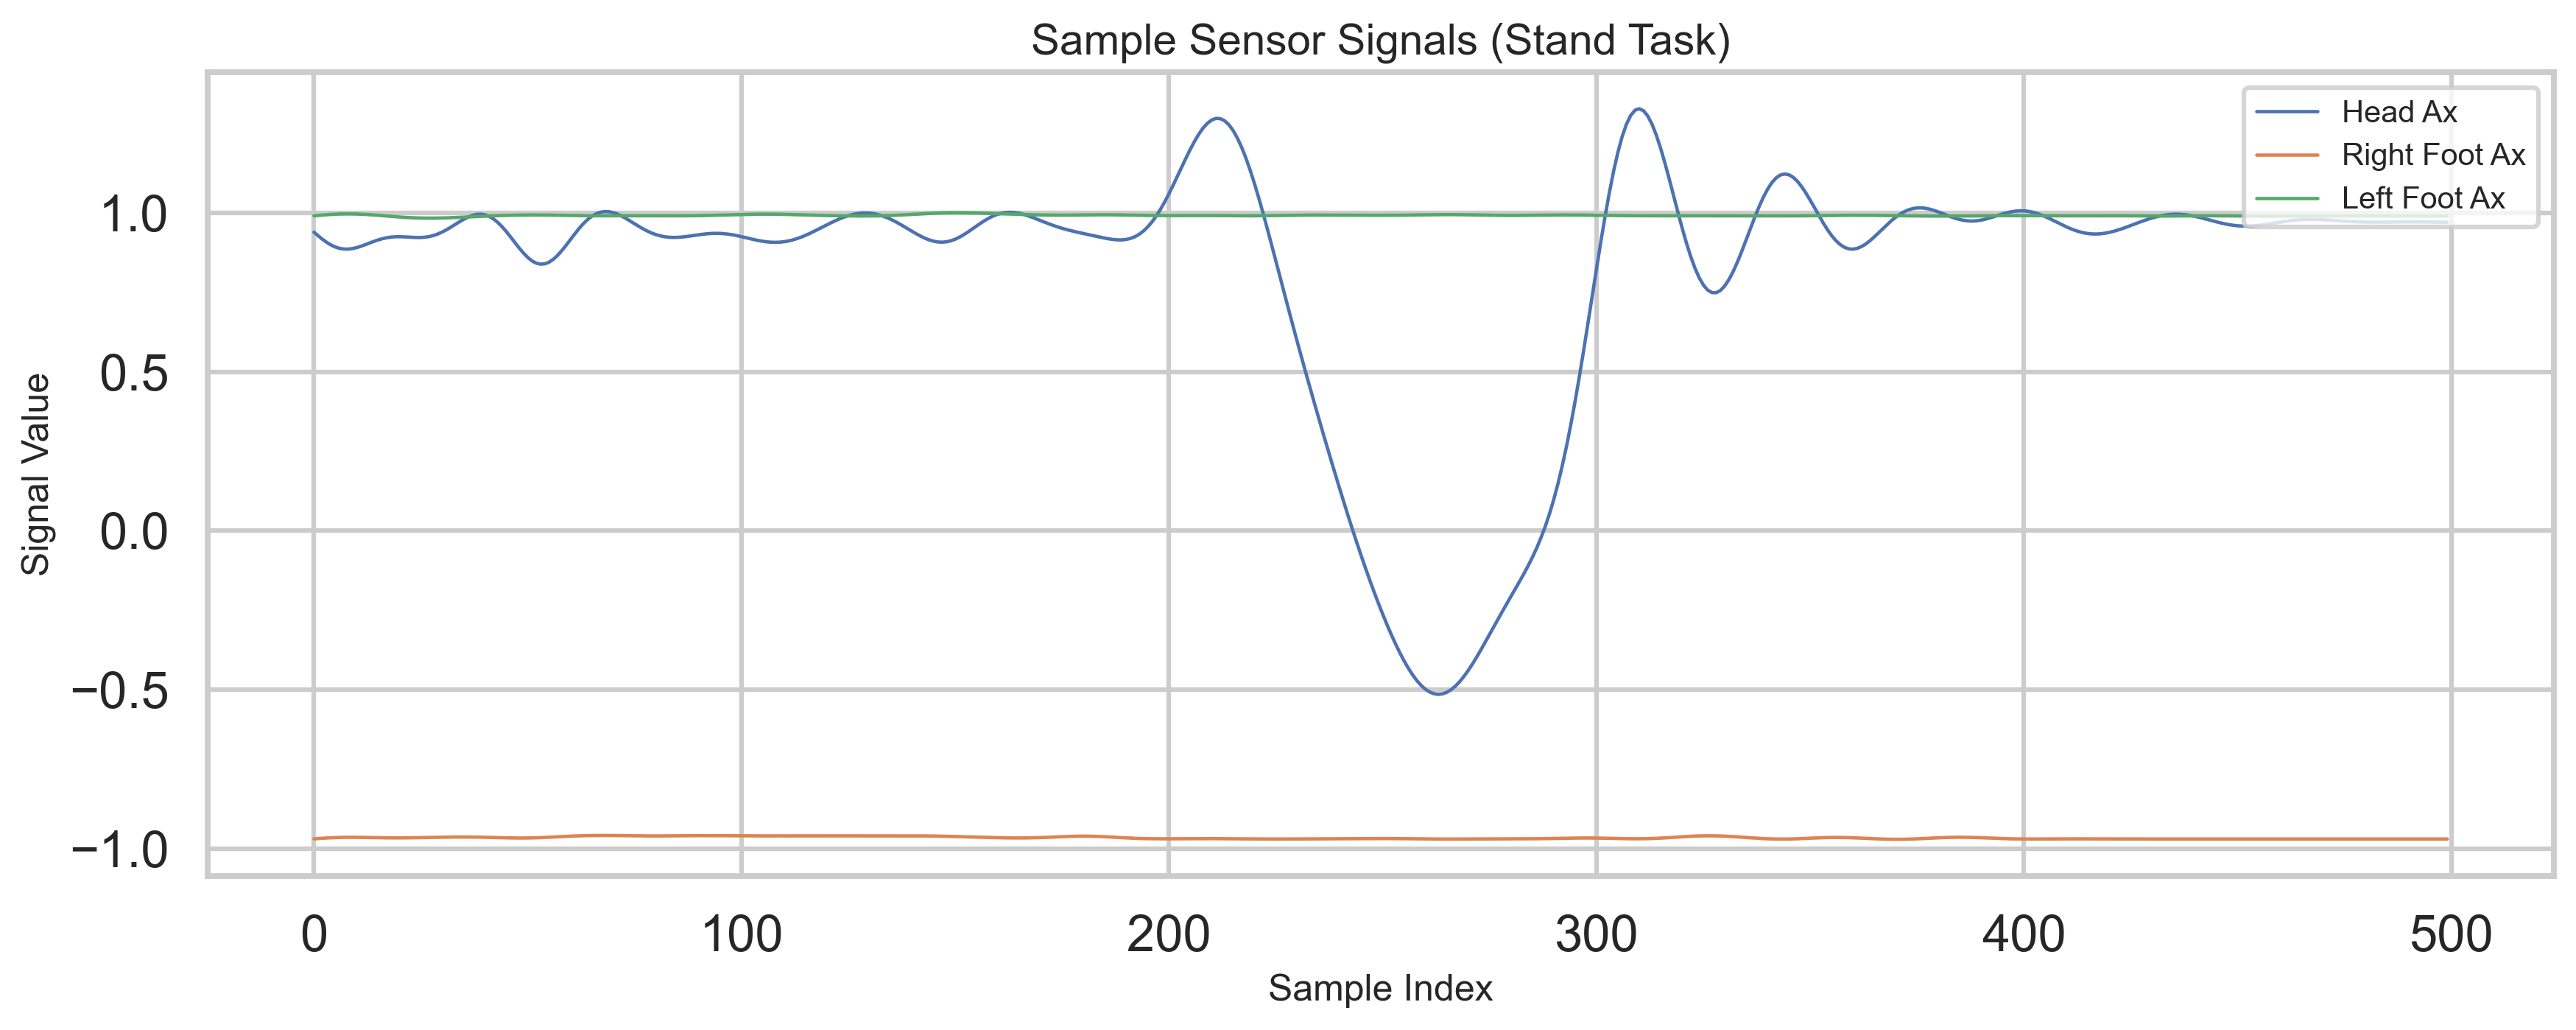
\includegraphics[width=0.85\linewidth]{Images/Generated/Chapter2/ch2_signal_sample.png}
	\caption{نمونه سیگنال های ثبت شده از حسگرها در فعالیت ایستادن}
	\label{fig:ch2_signal_sample}
\end{figure}


توزیع نمونه‌ها در کلاس‌های مختلف در
\autoref{fig:ch2_class_distribution}
نمایش داده شده است. همان‌گونه که مشاهده می‌شود، تمامی کلاس‌ها دارای تعداد یکسانی از نمونه‌ها هستند و برای هر کلاس ۲۵ نمونه در مجموعه داده در نظر گرفته شده است. متوازن بودن مجموعه داده موجب می‌شود عملکرد مدل‌ها تحت تأثیر عدم تعادل کلاس‌ها قرار نگیرد و معیارهایی مانند
  \lr{Accuracy}, \lr{Precision}, \lr{Recall}
 و
 \lr{F1}
  تصویر قابل اعتمادتری از عملکرد واقعی مدل‌ها ارائه دهند.

\begin{figure}[H]
	\centering
	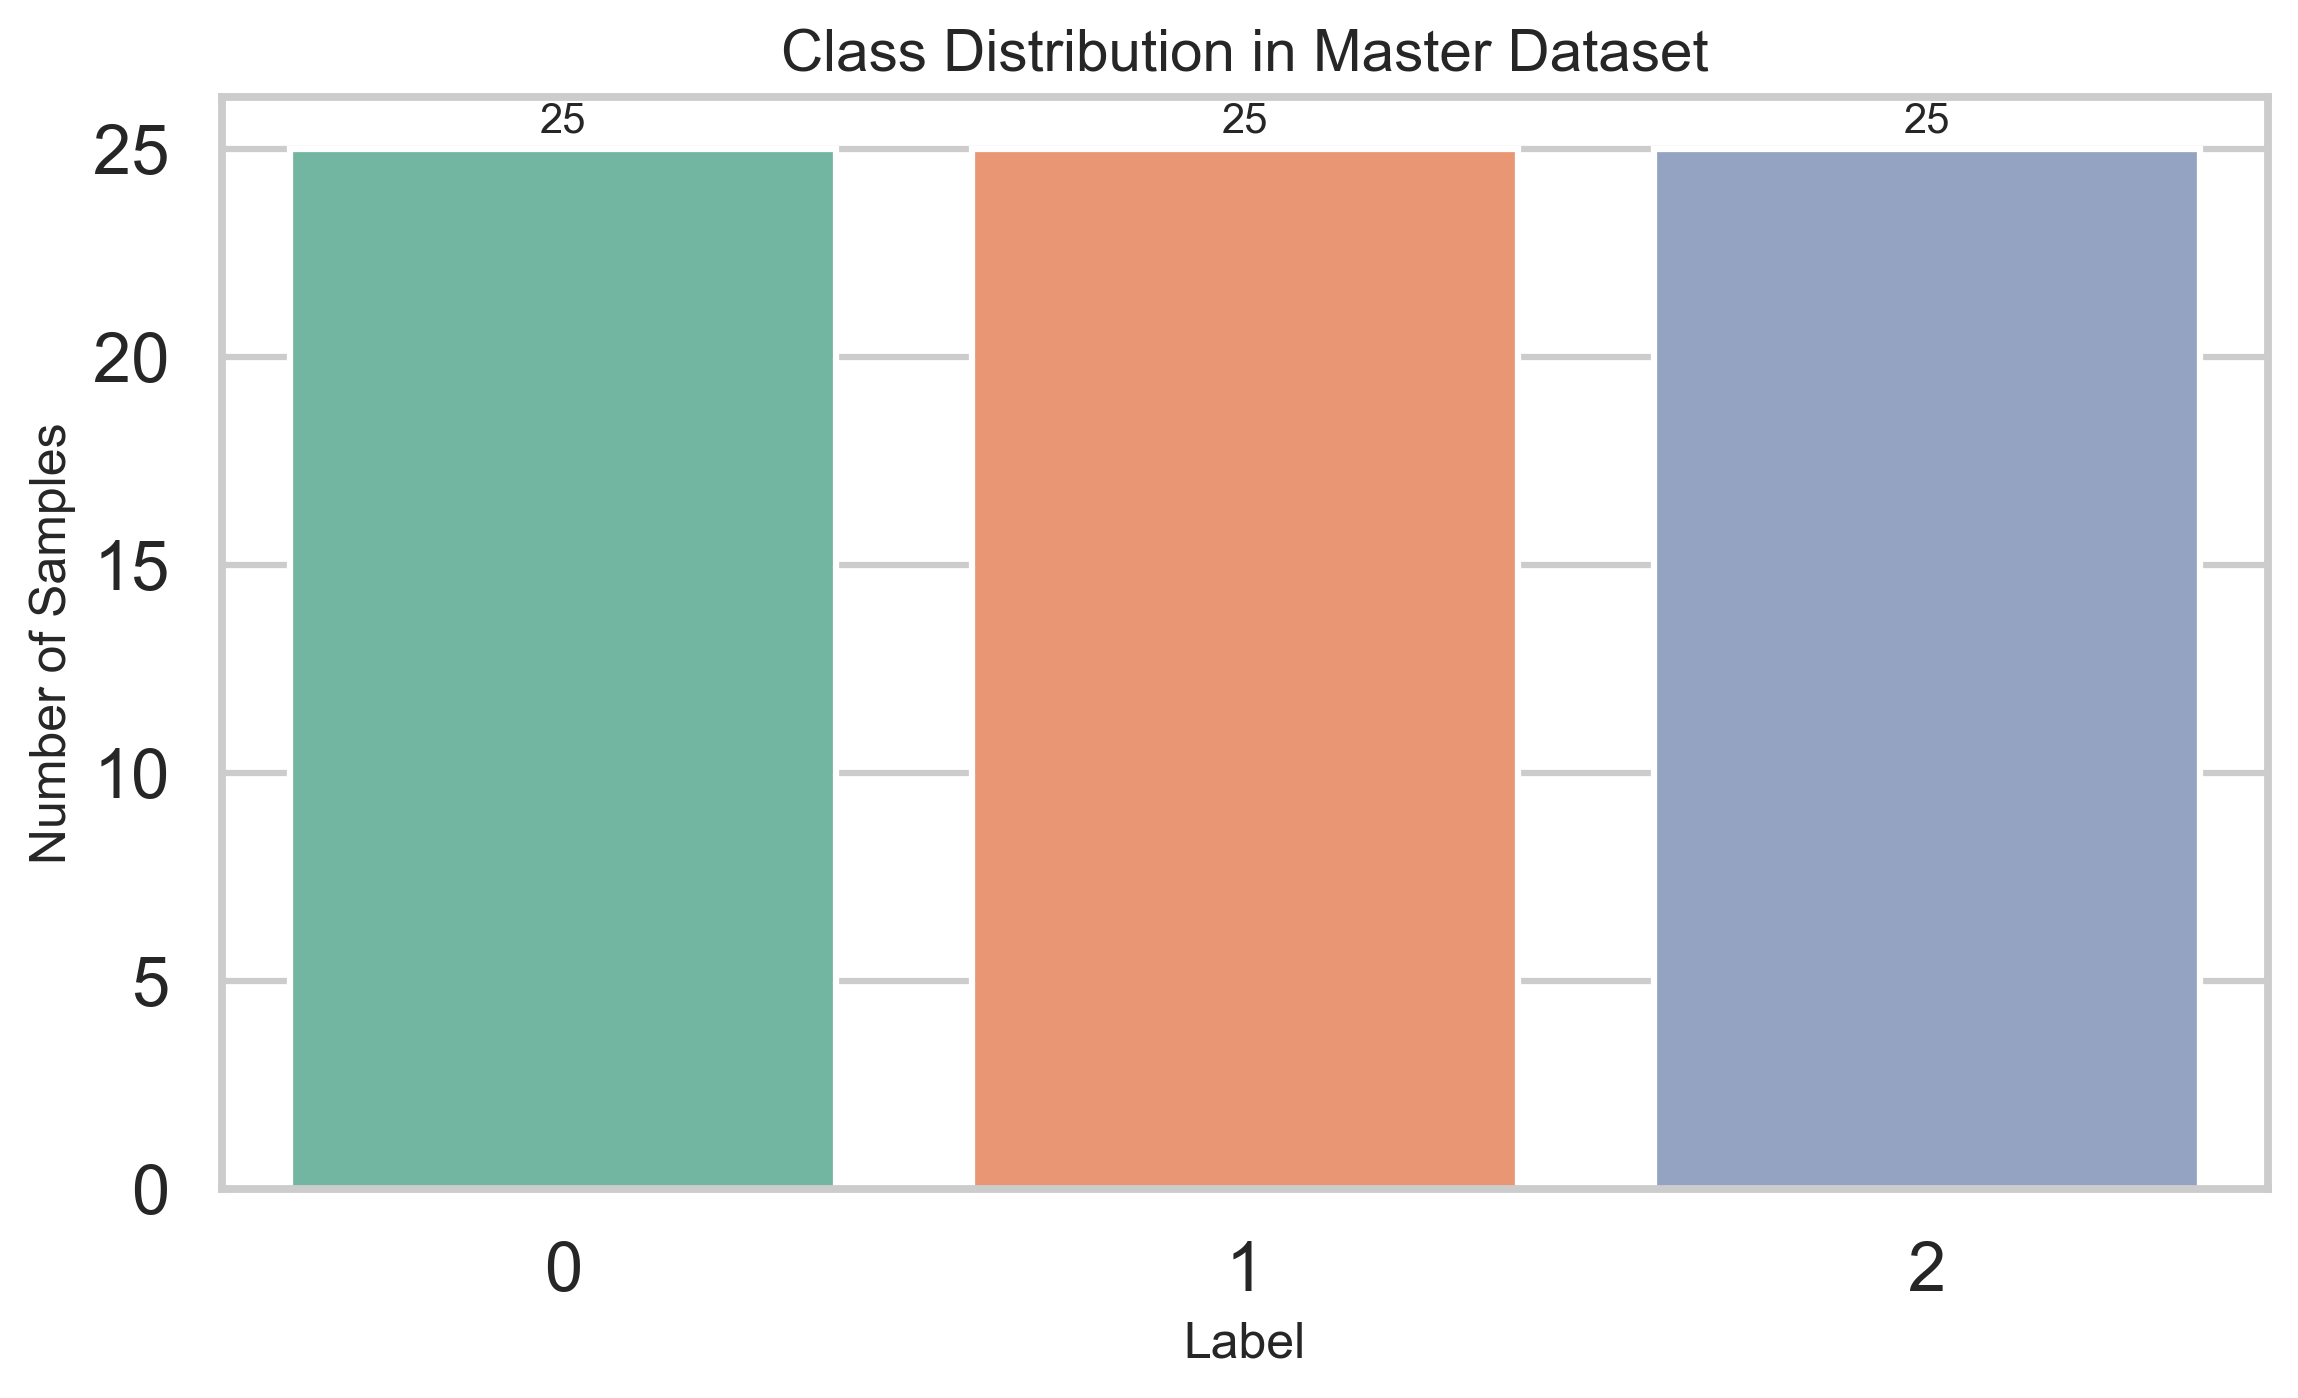
\includegraphics[width=0.85\linewidth]{Images/Generated/Chapter2/ch2_class_distribution.png}
	\caption{توزیع تعداد نمونه ها در کلاس های برچسب گذاری شده}
	\label{fig:ch2_class_distribution}
\end{figure}


\subsection{نتایج پیش‌پردازش داده‌ها}

پس از بررسی اولیه مجموعه داده، مراحل پیش‌پردازش شامل فیلترگذاری، حذف نویز و آماده‌سازی داده‌ها انجام شد. هدف از این مرحله افزایش کیفیت سیگنال‌ها و آماده‌سازی آن‌ها برای استخراج ویژگی بود.

یکی از بررسی‌های انجام‌شده پس از استخراج ویژگی‌ها، تحلیل میزان همبستگی بین ویژگی‌ها بود. همان‌طور که در 
 \autoref{fig:ch2_feature_correlation}
مشاهده می‌شود، تعدادی از ویژگی‌ها دارای همبستگی نسبتاً بالایی هستند که وجود اطلاعات تکراری در فضای ویژگی را نشان می‌دهد. این موضوع استفاده از روش‌های کاهش بعد مانند
 \lr{PCA}
 را توجیه می‌کند.
 
 \begin{figure}[H]
 	\centering
 	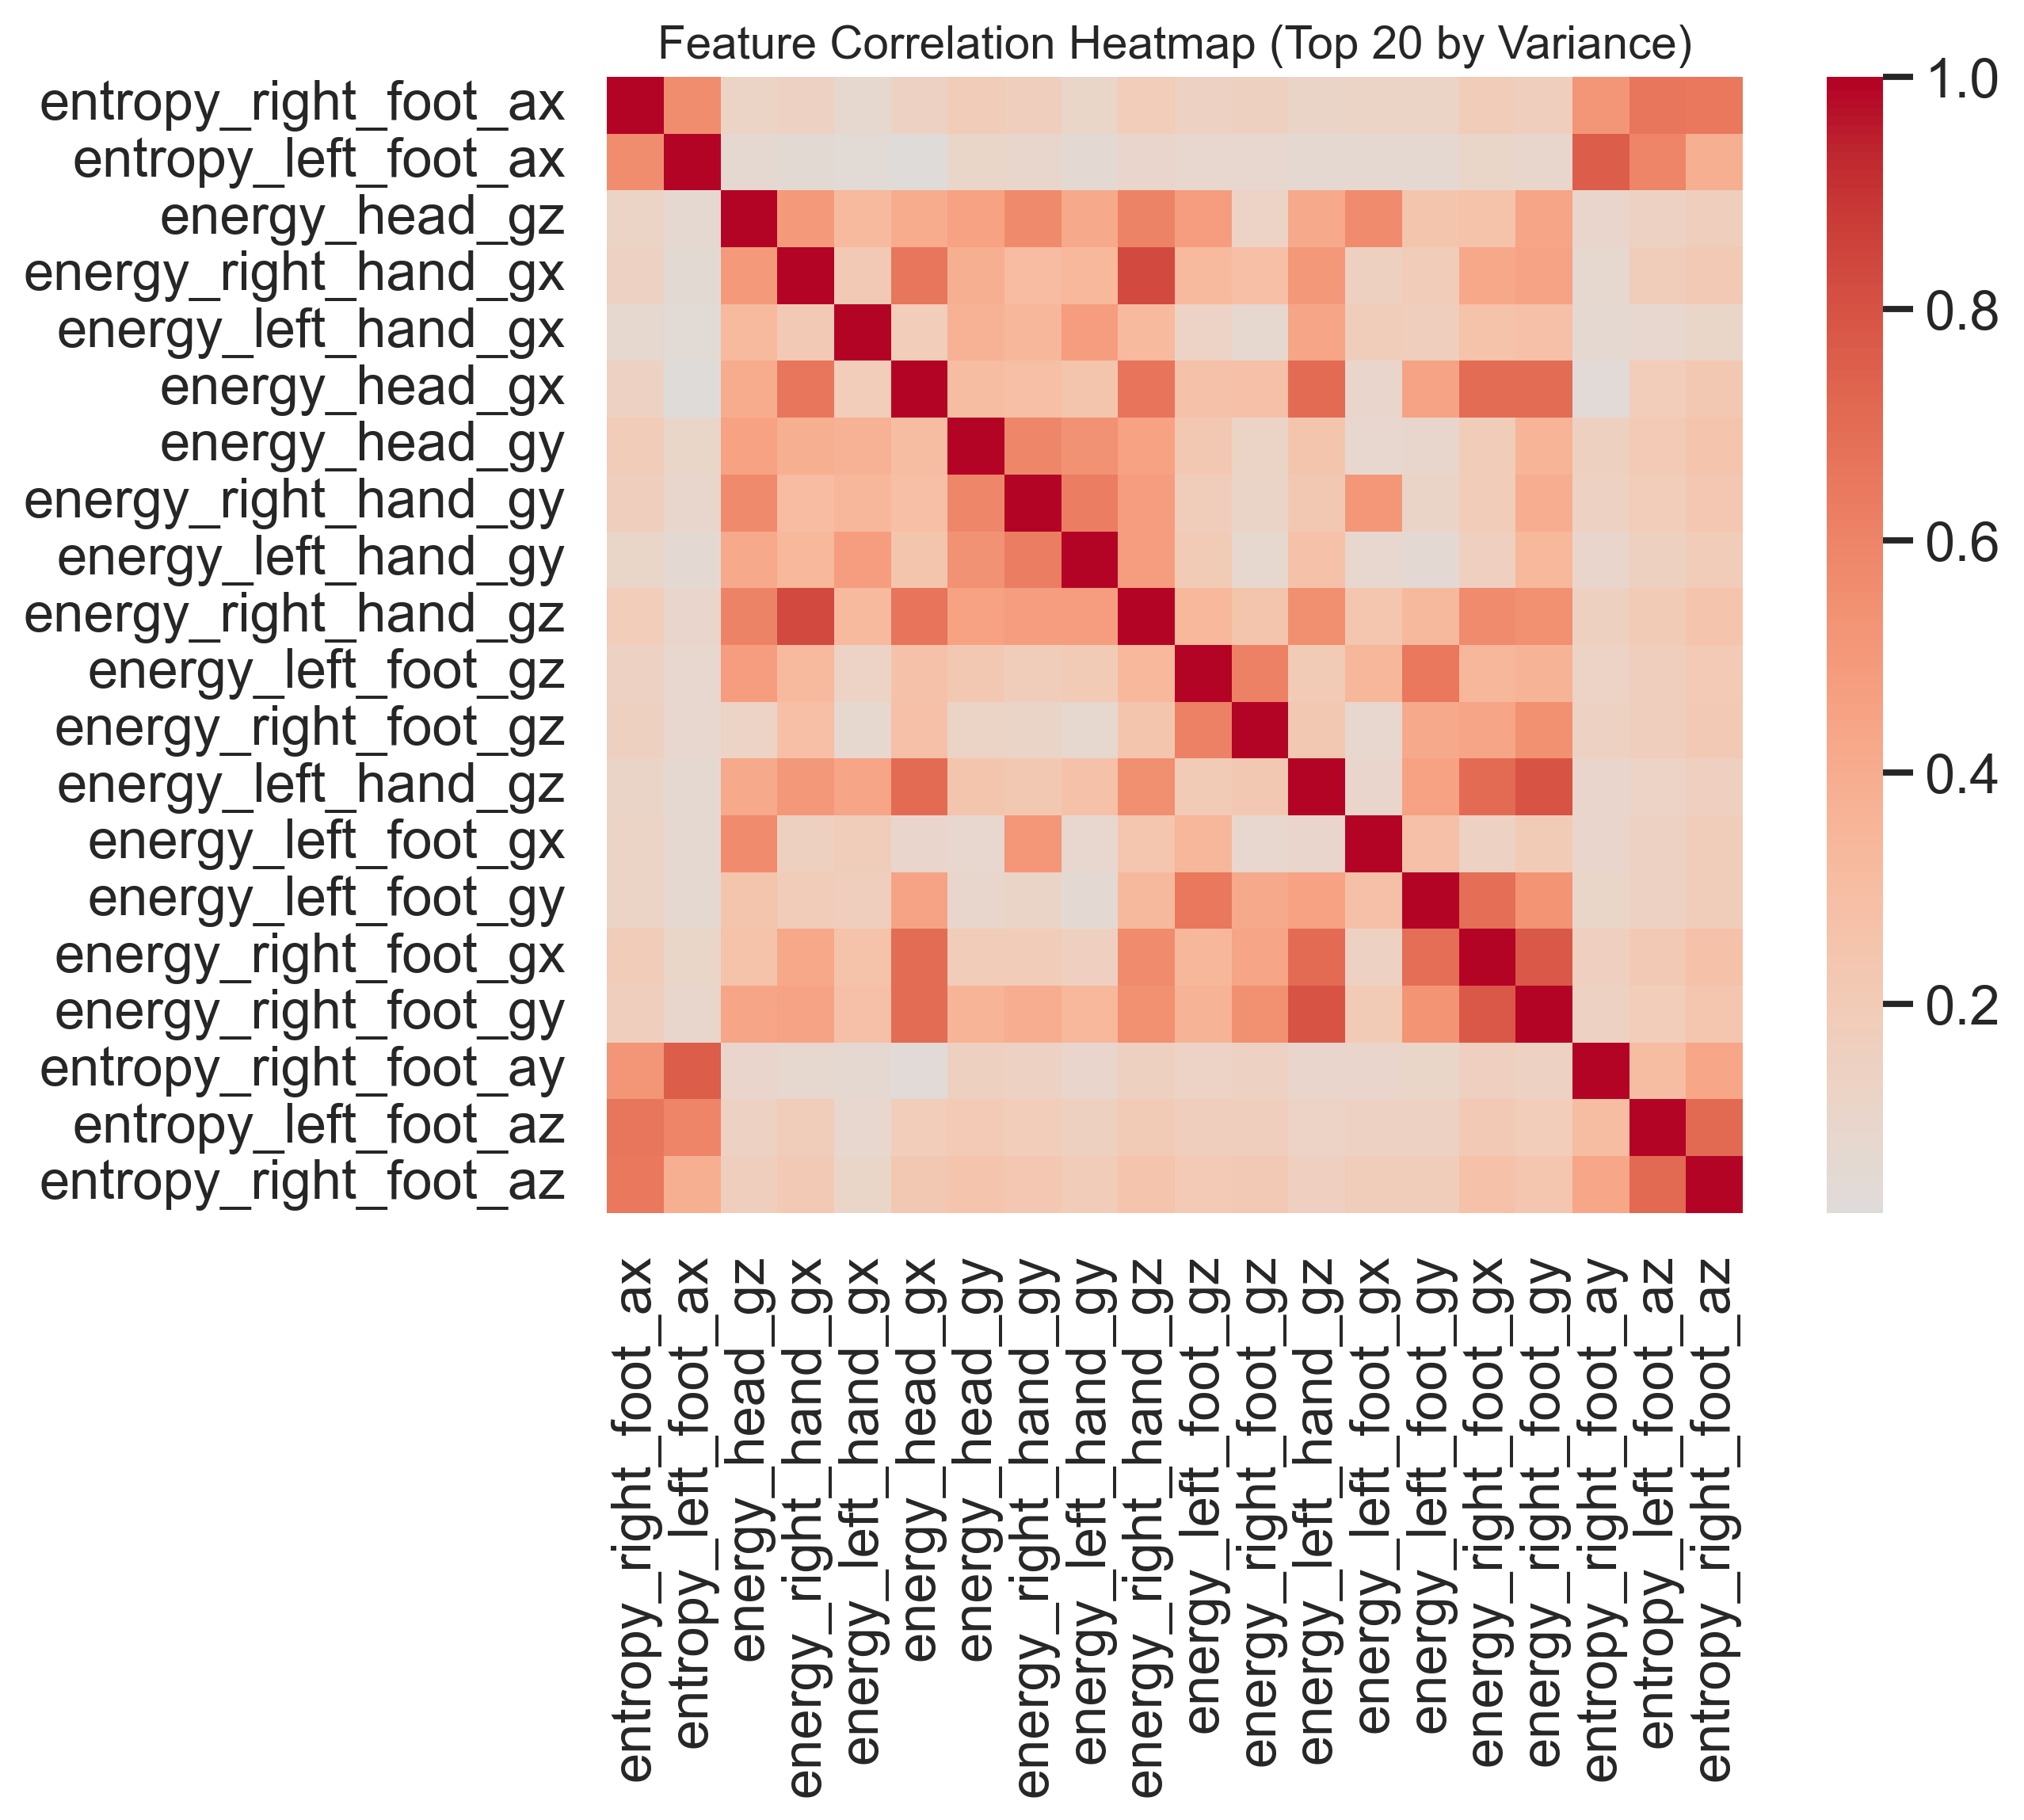
\includegraphics[width=0.85\linewidth]{Images/Generated/Chapter2/ch2_feature_correlation_heatmap.png}
 	\caption{نقشه همبستگی 20 ویژگی با بیشترین واریانس}
 	\label{fig:ch2_feature_correlation}
 \end{figure}
 
 
 \subsection{نتایج استخراج ویژگی}
 
پس از اعمال مراحل پیش‌پردازش، مجموعه‌ای از ویژگی‌های آماری و حوزه زمان از سیگنال‌های ثبت‌شده استخراج شد. این ویژگی‌ها اطلاعات مختلفی از رفتار دینامیکی حرکت آزمودنی را توصیف می‌کنند و به عنوان ورودی مدل‌های یادگیری ماشین مورد استفاده قرار گرفتند.

با توجه به اینکه تعداد ویژگی‌های استخراج‌شده نسبتاً زیاد بود، پیش از آموزش مدل‌ها ساختار فضای ویژگی مورد بررسی قرار گرفت. نتایج نشان داد بخشی از ویژگی‌ها دارای همبستگی قابل توجهی با یکدیگر هستند که نشان‌دهنده وجود اطلاعات تکراری در داده‌ها است. این موضوع یکی از دلایل اصلی بررسی روش کاهش بعد با استفاده از 
\lr{PCA}
 در ادامه پژوهش محسوب می‌شود.


\subsection{نتایج مدل‌های یادگیری ماشین}

سه مدل مختلف شامل 
\lr{KNN}، \lr{SVM}
 و
 \lr{Random Forest}
 برای پیش‌بینی کلاس فعالیت آموزش داده شدند. عملکرد این مدل‌ها با استفاده از معیارهای
 \lr{Accuracy}، \lr{Precision}، \lr{Recall} 
  و
 \lr{F1}
    مورد ارزیابی قرار گرفت.


\begin{figure}[H]
	\centering
	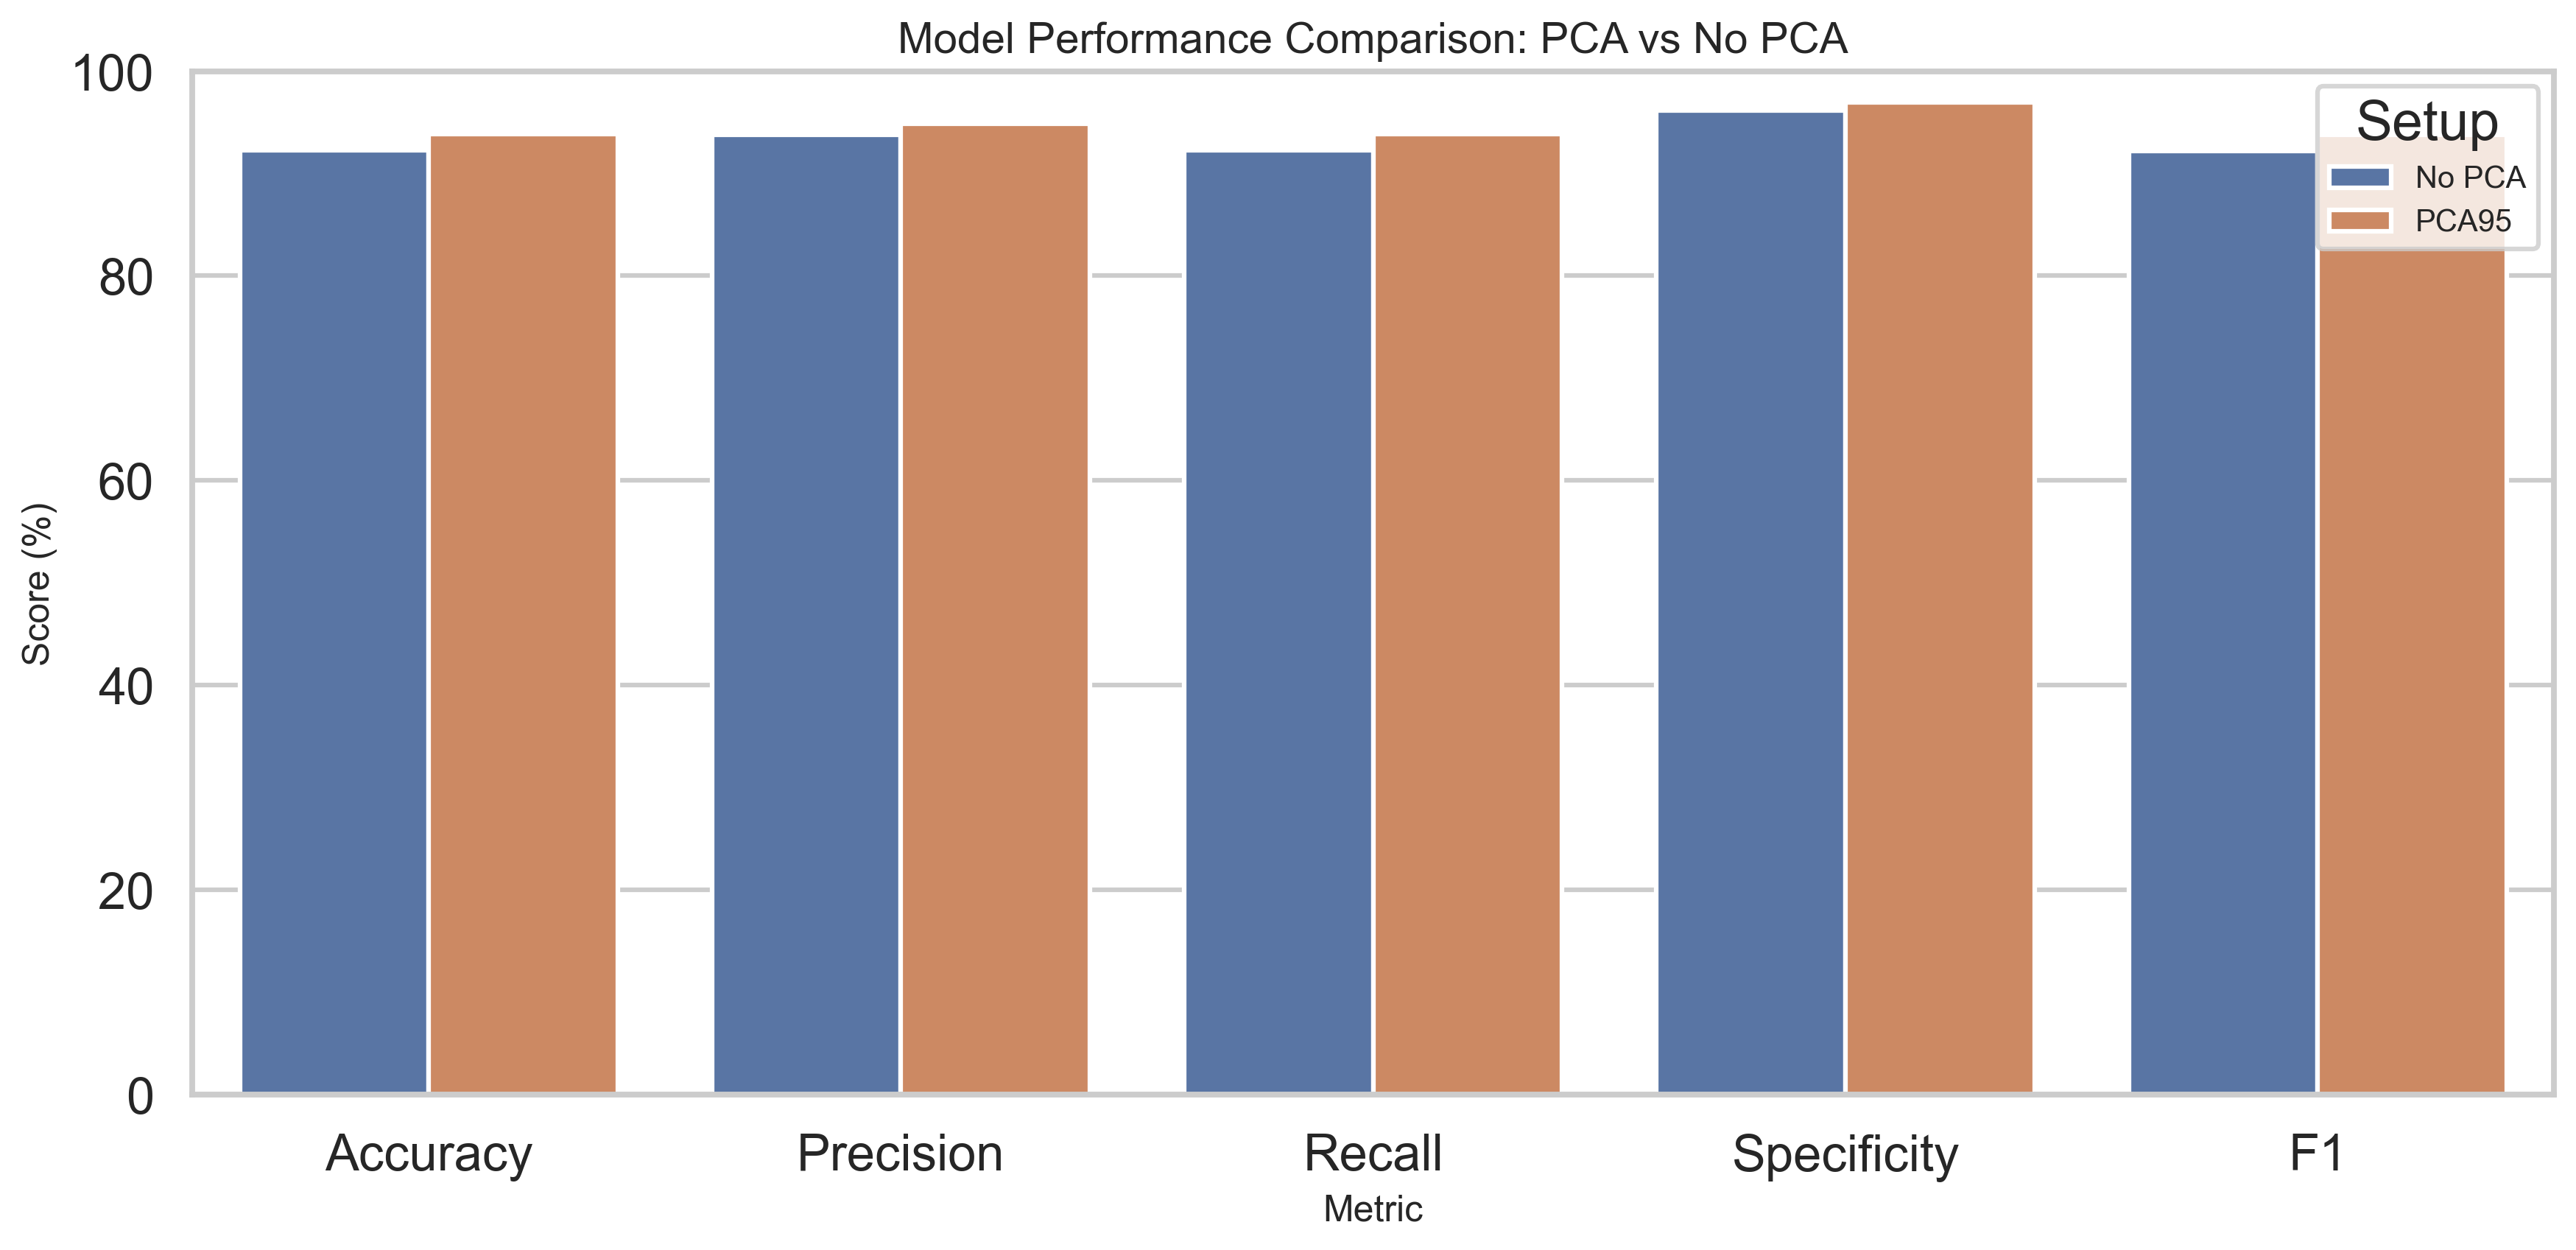
\includegraphics[width=0.85\linewidth]{Images/Generated/Chapter3/ch3_metrics_pca_vs_no_pca.png}
	\caption{مقایسه معیارهای عملکرد مدل ها در دو حالت بدون \lr{PCA} و با \lr{PCA95}}
	\label{fig:ch3_metrics_pca_vs_no_pca}
\end{figure}

مطابق شکل \ref{fig:ch3_metrics_pca_vs_no_pca}، عملکرد مدل‌های مختلف در دو حالت استفاده از ویژگی‌های اولیه و ویژگی‌های کاهش‌یافته مقایسه شده است. این نمودار امکان بررسی اثر کاهش بعد بر هر یک از الگوریتم‌ها را فراهم می‌کند و نشان می‌دهد که واکنش مدل‌های مختلف نسبت به اعمال 
\lr{PCA}
 یکسان نیست.



علاوه بر معیارهای عددی، برای بررسی دقیق‌تر نوع خطاهای مدل‌ها از ماتریس درهم‌ریختگی نرمال‌شده استفاده شد. این ماتریس‌ها نشان می‌دهند که هر مدل در تشخیص کدام کلاس‌ها عملکرد مناسب‌تری داشته و بیشترین اشتباهات بین کدام کلاس‌ها رخ داده است.

\begin{figure}[H]
	\centering
	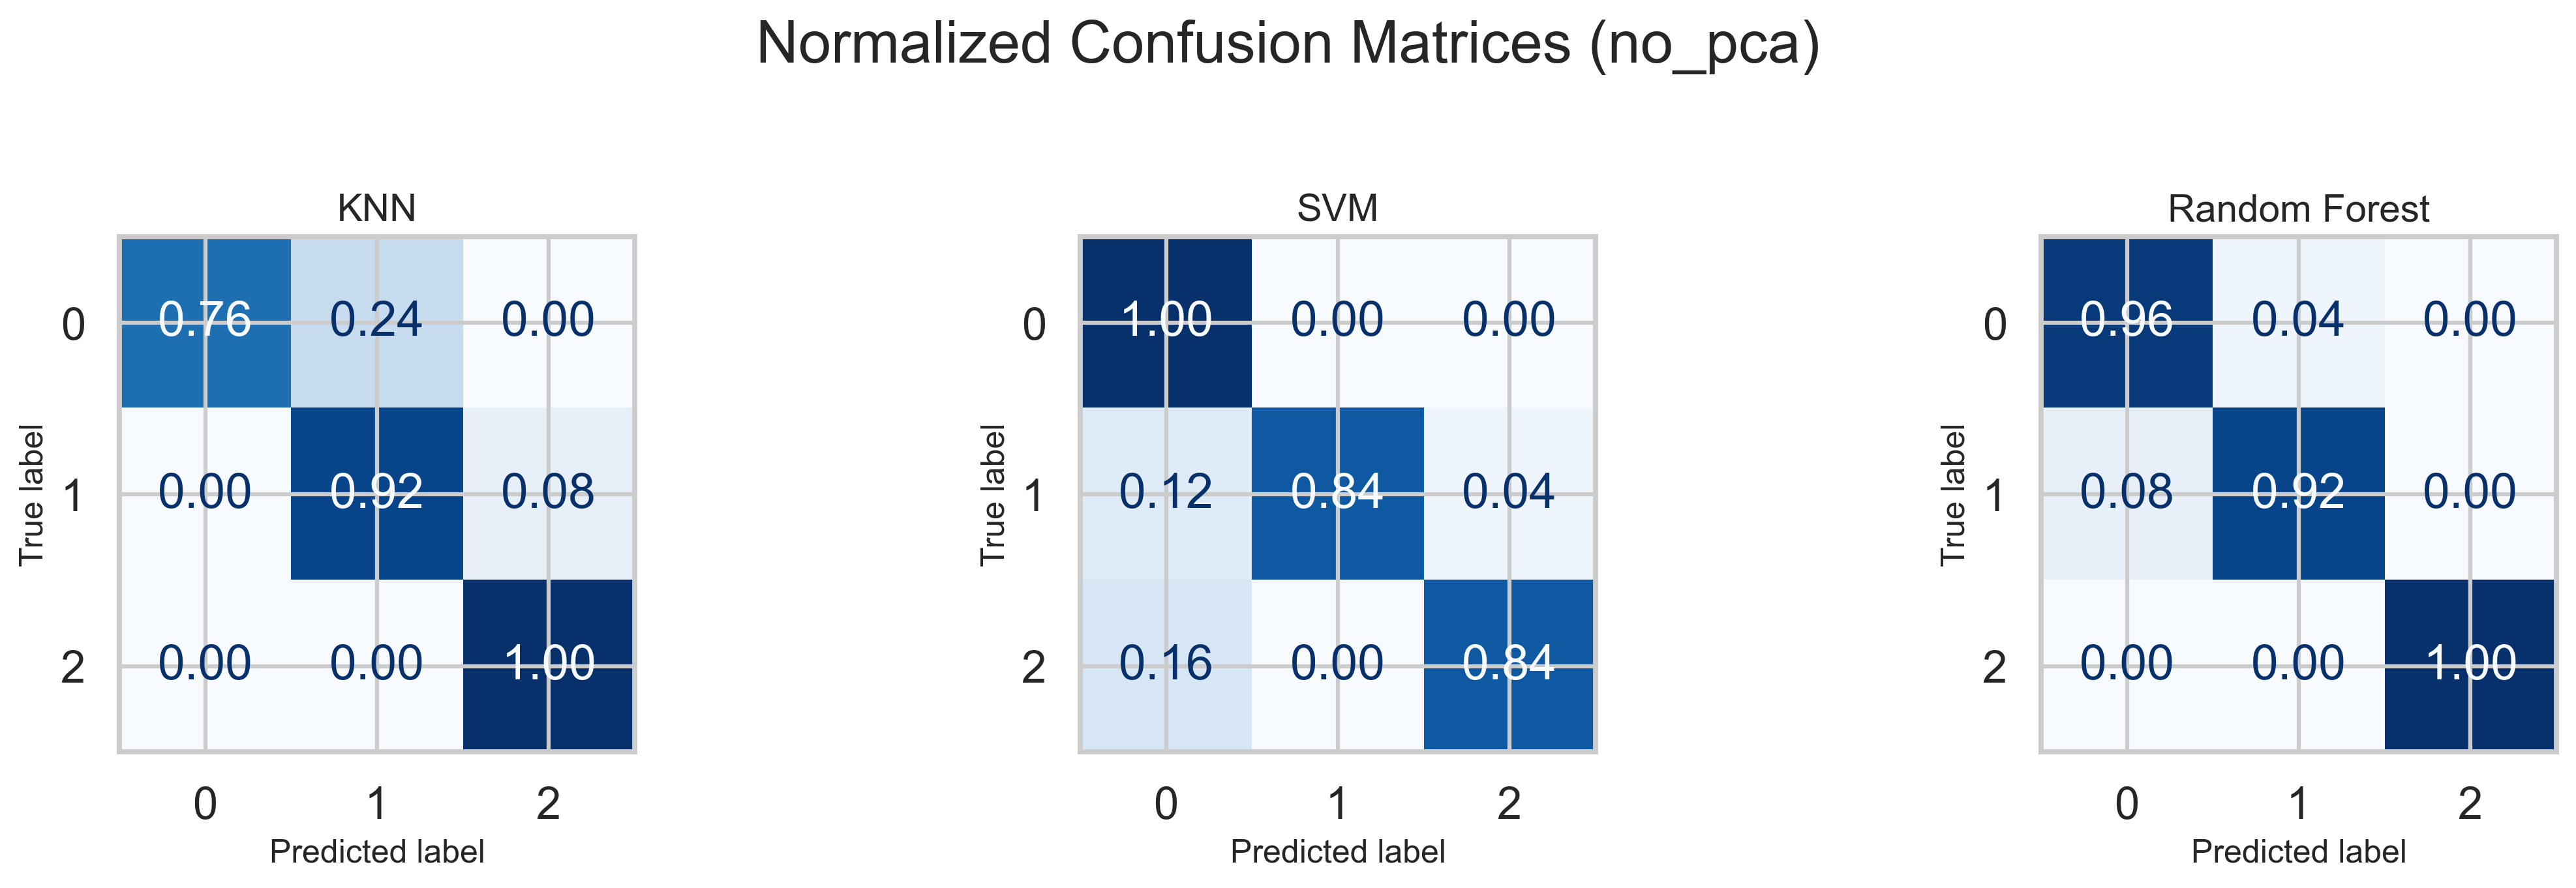
\includegraphics[width=0.85\linewidth]{Images/Generated/Chapter3/ch3_confusion_matrices_no_pca.png}
	\caption{ماتریس درهم ریختگی نرمال شده مدل ها در حالت \lr{no pca}}
	\label{fig:ch3_confusion_no_pca}
\end{figure}

\noindent\textbf{توضیح شکل:} این شکل خطاهای بین کلاسی را مشخص می کند و نشان می دهد هر مدل کدام کلاس ها را بهتر یا ضعیف تر تشخیص می دهد.
\vspace{0.8em}

\begin{figure}[H]
	\centering
	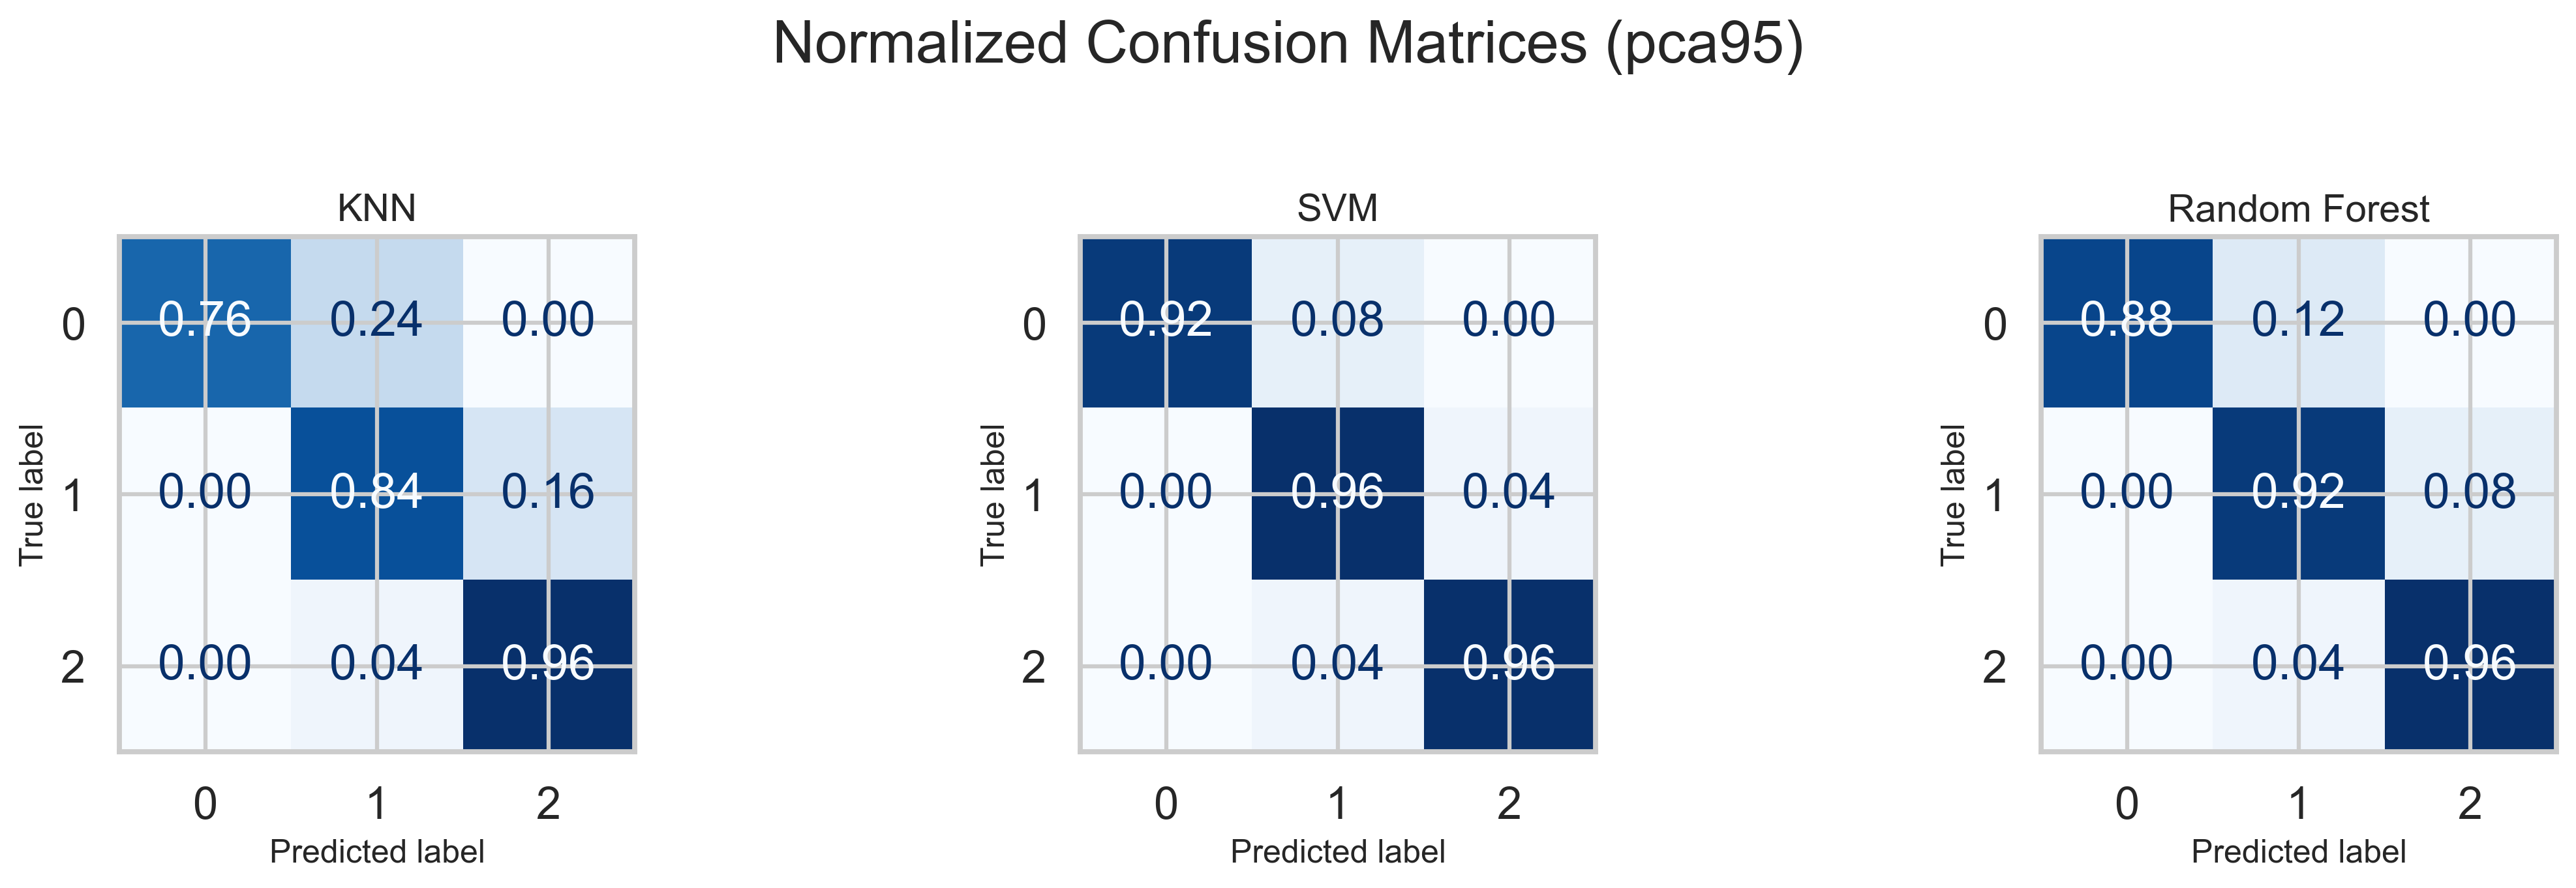
\includegraphics[width=0.85\linewidth]{Images/Generated/Chapter3/ch3_confusion_matrices_pca95.png}
	\caption{ماتریس درهم ریختگی نرمال شده مدل ها در حالت \lr{pca95}}
	\label{fig:ch3_confusion_pca95}
\end{figure}

\noindent\textbf{توضیح شکل:} این شکل خطاهای بین کلاسی را مشخص می کند و نشان می دهد هر مدل کدام کلاس ها را بهتر یا ضعیف تر تشخیص می دهد.
\vspace{0.8em}

\begin{figure}[H]
	\centering
	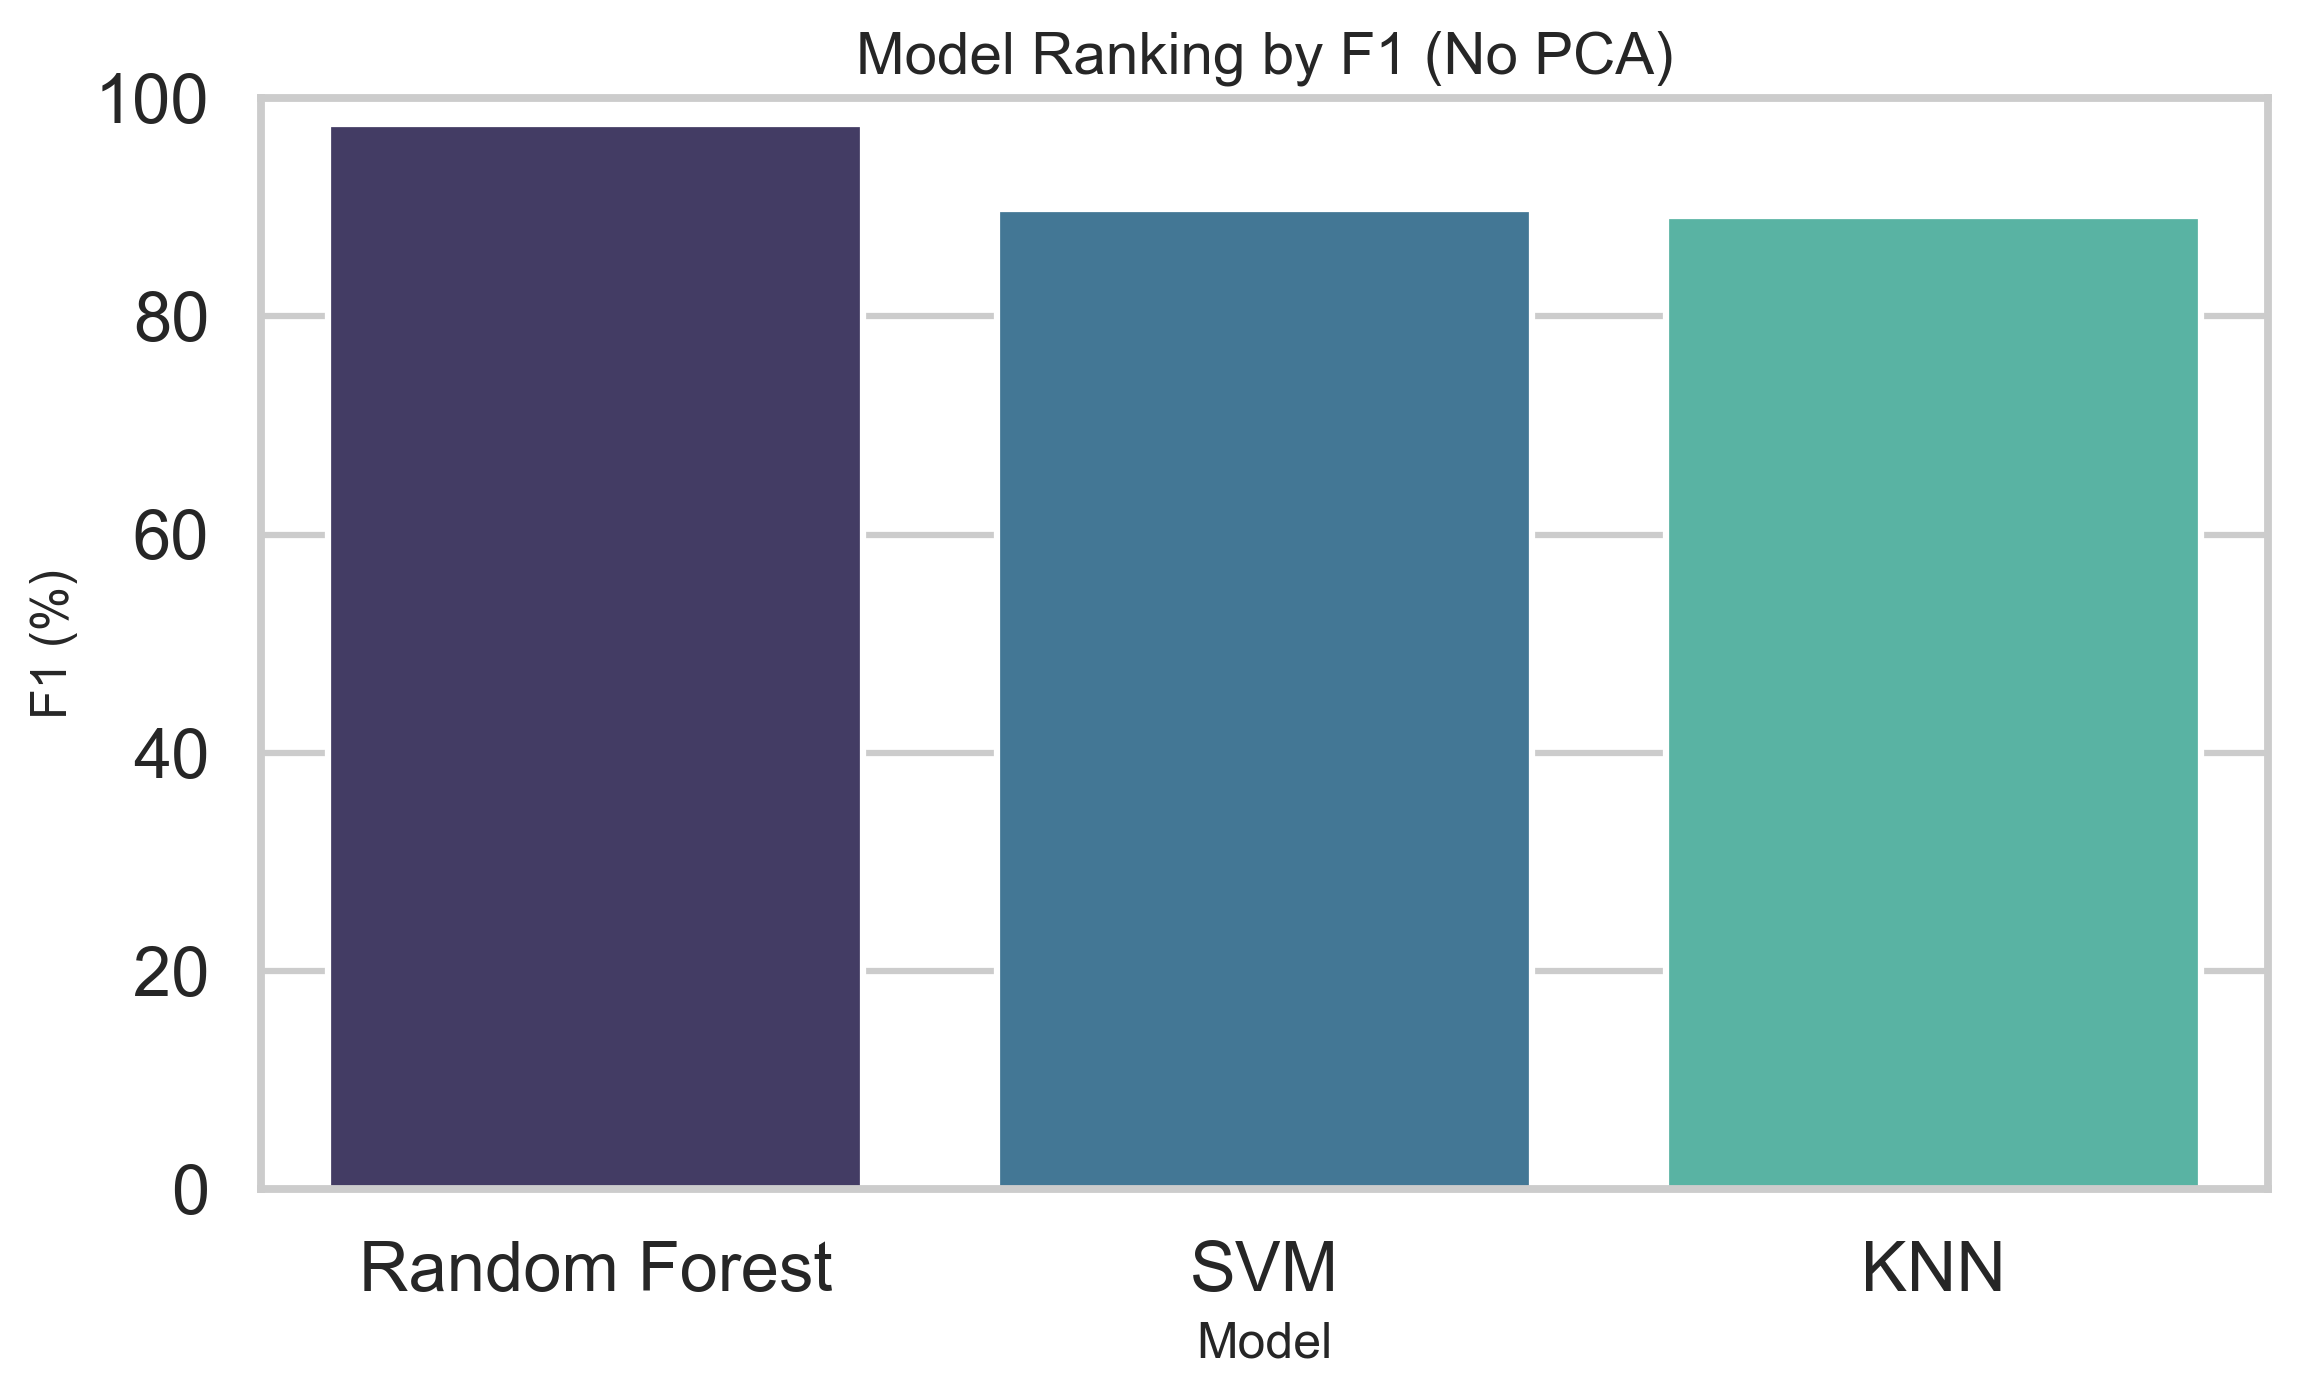
\includegraphics[width=0.85\linewidth]{Images/Generated/Chapter3/ch3_model_ranking_f1_no_pca.png}
	\caption{رتبه بندی مدل ها بر اساس \lr{F1} در حالت بدون \lr{PCA}}
	\label{fig:ch3_model_ranking}
\end{figure}

\noindent\textbf{توضیح شکل:} این شکل جمع بندی سریع از برتری نسبی مدل ها ارائه می دهد و انتخاب مدل نهایی را پشتیبانی می کند.
\vspace{0.8em}

\begin{table}[H]
	\centering
	\caption{مقایسه عملکرد مدل‌های مختلف}
	\label{tab:model_results}
	
	\begin{tabular}{lcccc}
		\toprule
		مدل &
		\lr{Accuracy} &
		\lr{Precision} &
		\lr{Recall} &
		\lr{F1-score}\\
		\midrule
		\lr{KNN} & & & & \\
		\lr{SVM} & & & & \\
		\lr{Random Forest} & & & & \\
		\bottomrule
	\end{tabular}
	
\end{table}


\subsection{تأثیر کاهش بعد با استفاده از \lr{PCA}}

به منظور بررسی اثر کاهش بعد بر عملکرد مدل‌ها، روش
 \lr{PCA}
 با حفظ 95 درصد واریانس داده‌ها مورد استفاده قرار گرفت. در این بخش نتایج حاصل از آموزش مدل‌ها قبل و بعد از اعمال
 \lr{PCA}
   مقایسه می‌شوند.
   
   در این پژوهش، تعداد مؤلفه‌های اصلی به گونه‌ای انتخاب شد که ۹۵ درصد از واریانس کل داده‌ها حفظ شود. به این ترتیب، بخش عمده اطلاعات موجود در داده‌ها بدون حفظ تمامی ویژگی‌های اولیه نگهداری شد.

\begin{figure}[H]
	\centering
	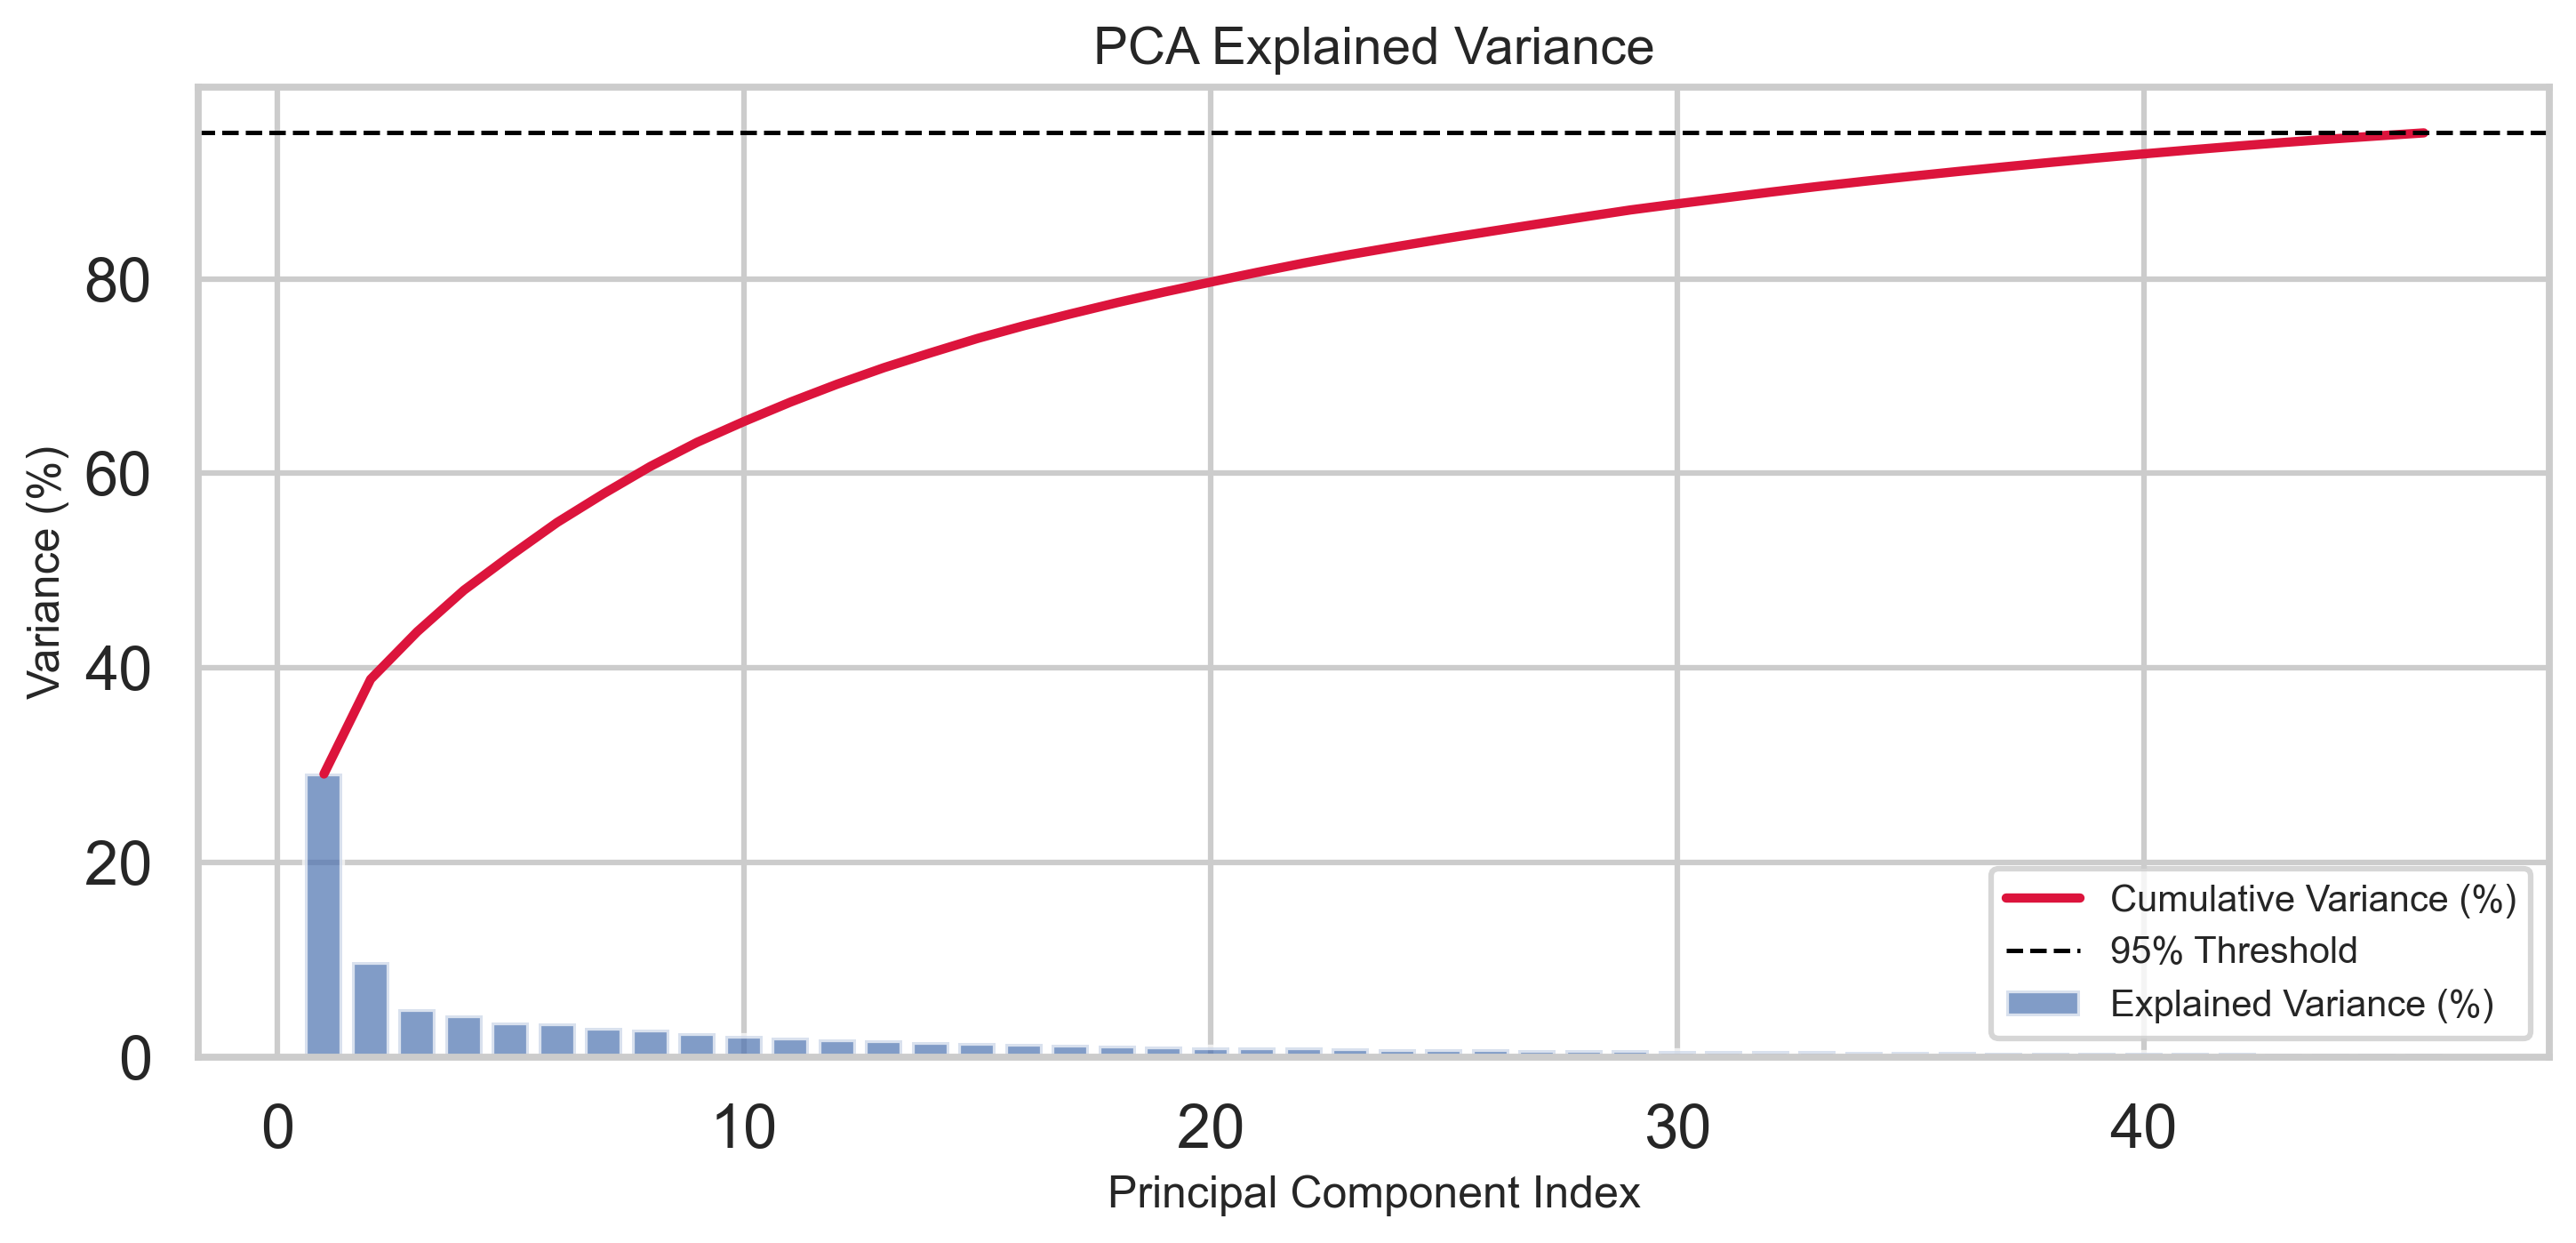
\includegraphics[width=0.85\linewidth]{Images/Generated/Chapter3/ch3_pca_variance_curve.png}
	\caption{درصد واریانس توضیح داده شده و تجمعی مولفه های اصلی}
	\label{fig:ch3_pca_variance}
\end{figure}

مطابق شکل \ref{fig:ch3_pca_variance} مشاهده می‌شود که با تعداد محدودی از مؤلفه‌های اصلی می‌توان بخش عمده واریانس داده‌ها را حفظ کرد. این موضوع بیانگر وجود همبستگی میان ویژگی‌های استخراج‌شده و امکان کاهش بعد بدون از دست رفتن بخش زیادی از اطلاعات است.


\begin{figure}[H]
	\centering
	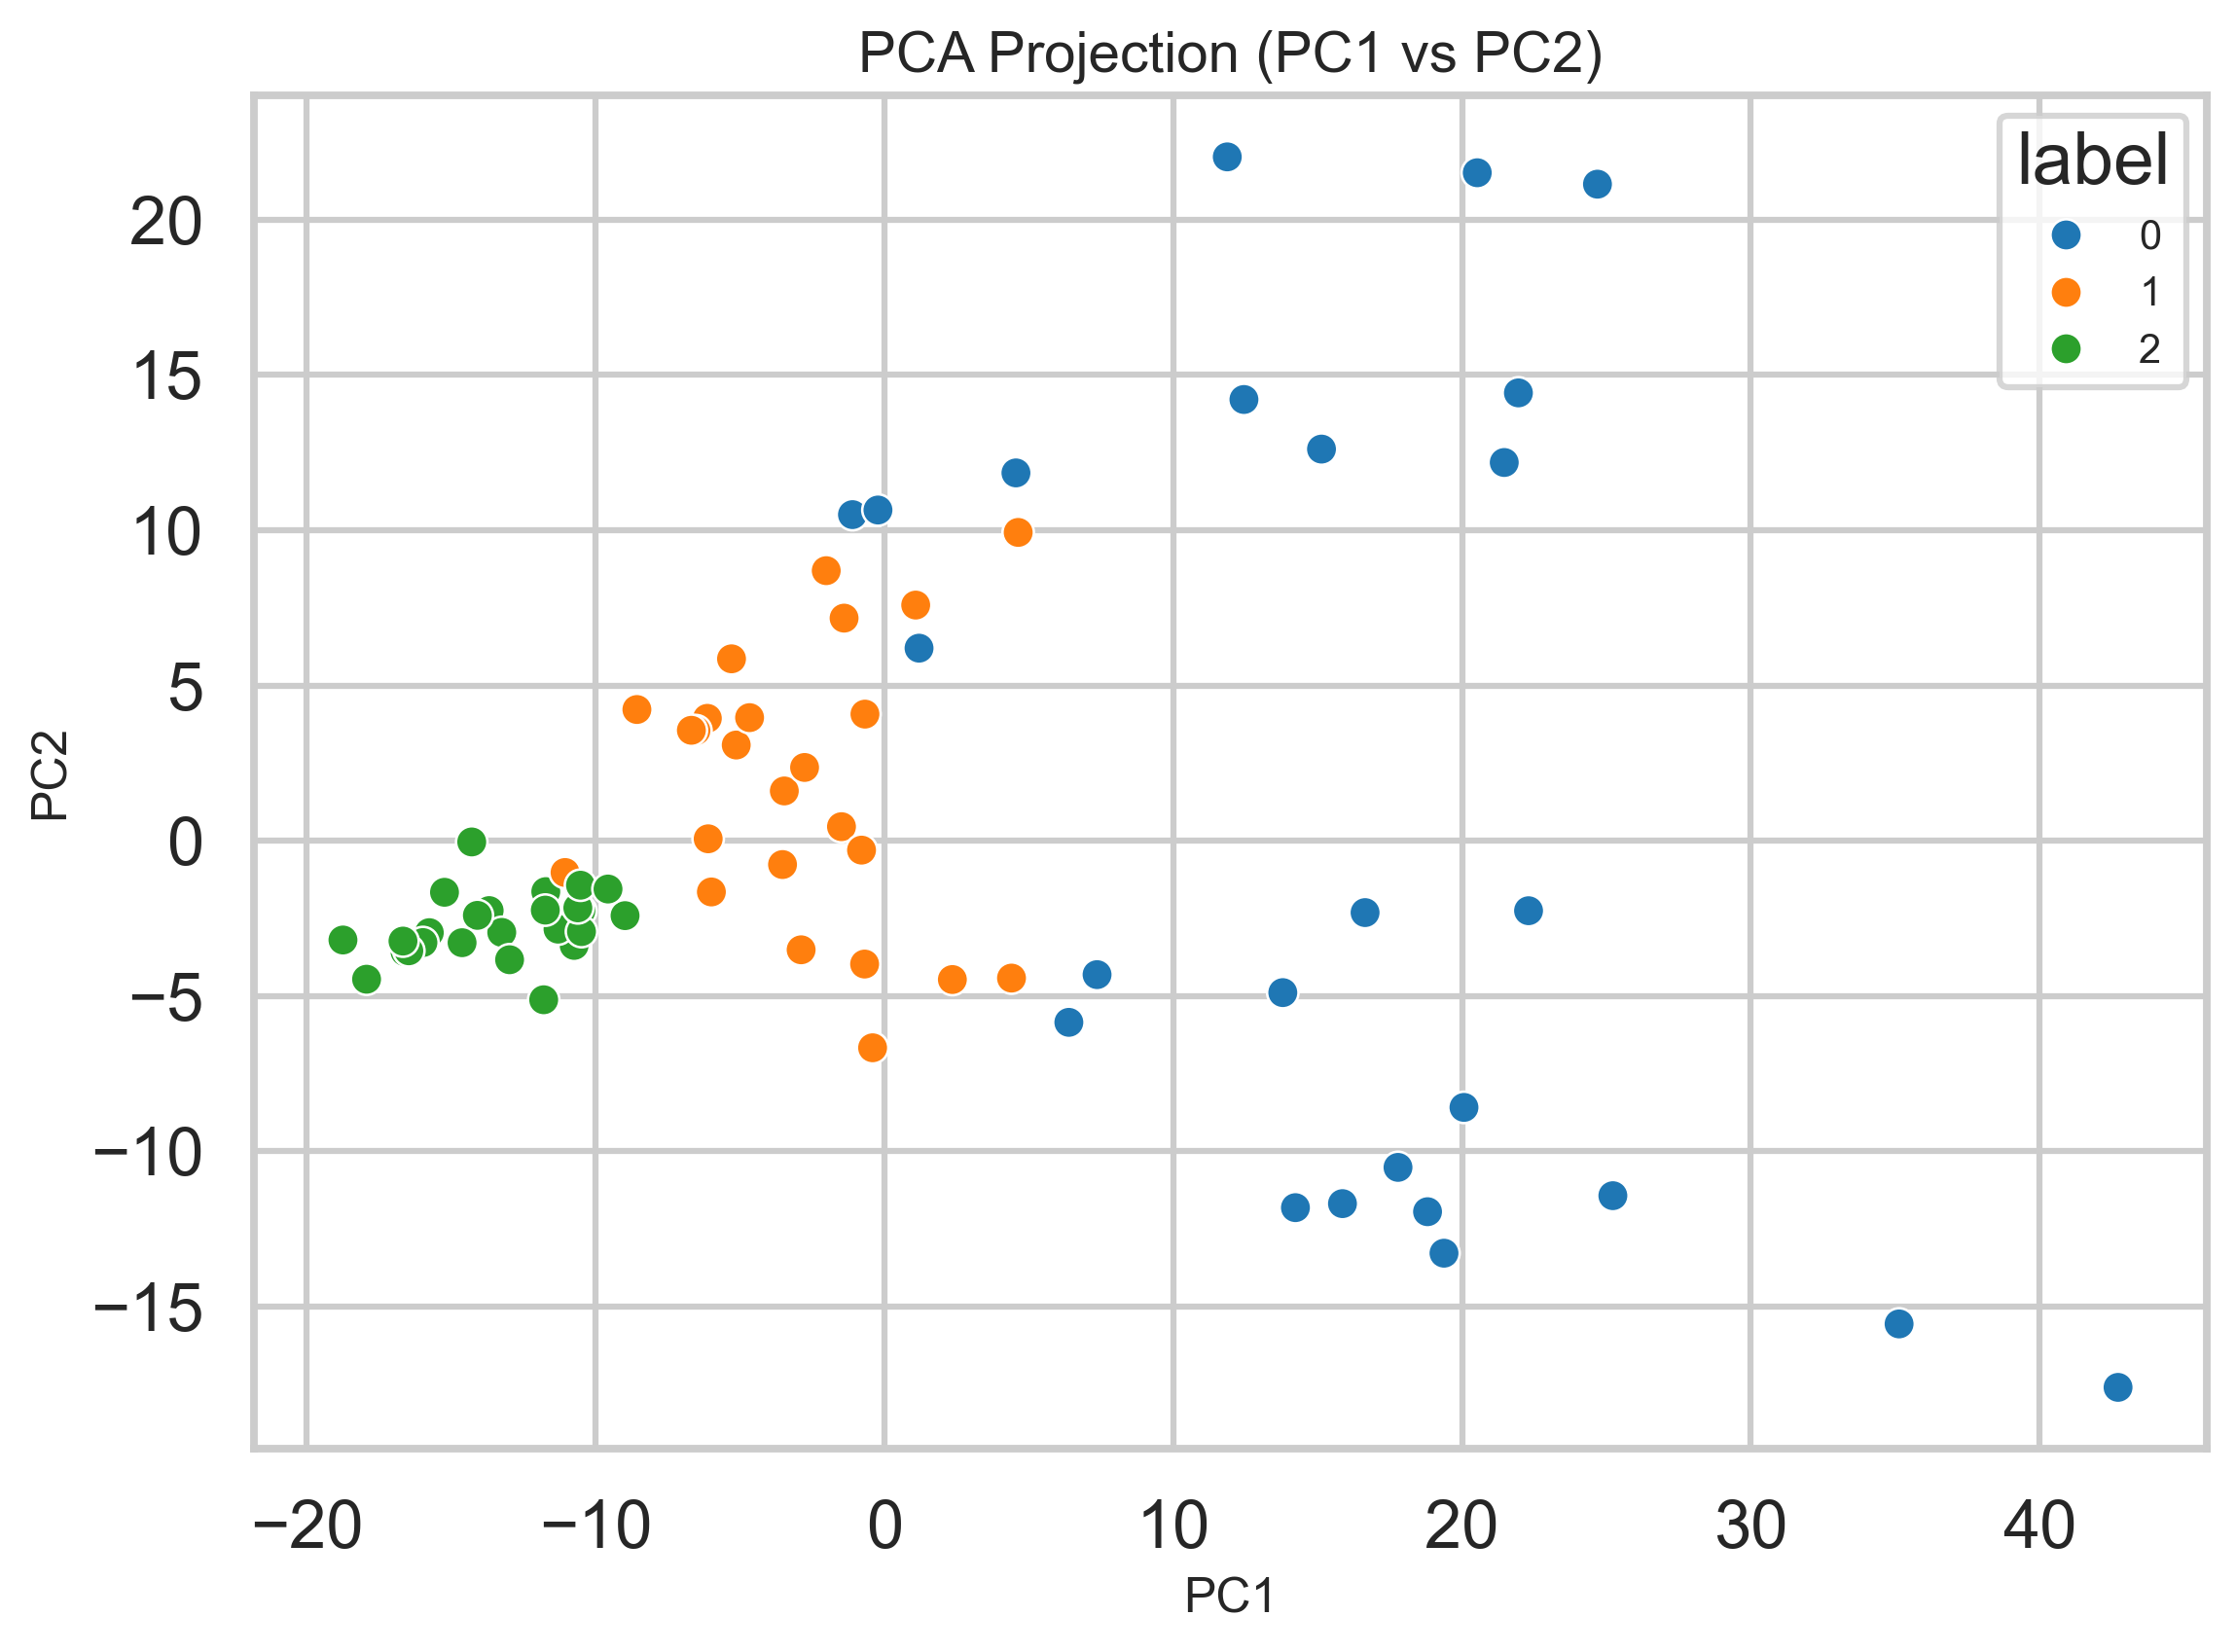
\includegraphics[width=0.85\linewidth]{Images/Generated/Chapter3/ch3_pca_scatter_pc1_pc2.png}
	\caption{پراکندگی نمونه ها در فضای \lr{PC1} و \lr{PC2}}
	\label{fig:ch3_pca_scatter}
\end{figure}

\noindent\textbf{توضیح شکل:} این نمودار میزان جداسازی کلاس ها را در فضای PCA نمایش می دهد و شهودی از دشواری طبقه بندی ارائه می کند.
\vspace{0.8em}

\begin{figure}[H]
	\centering
	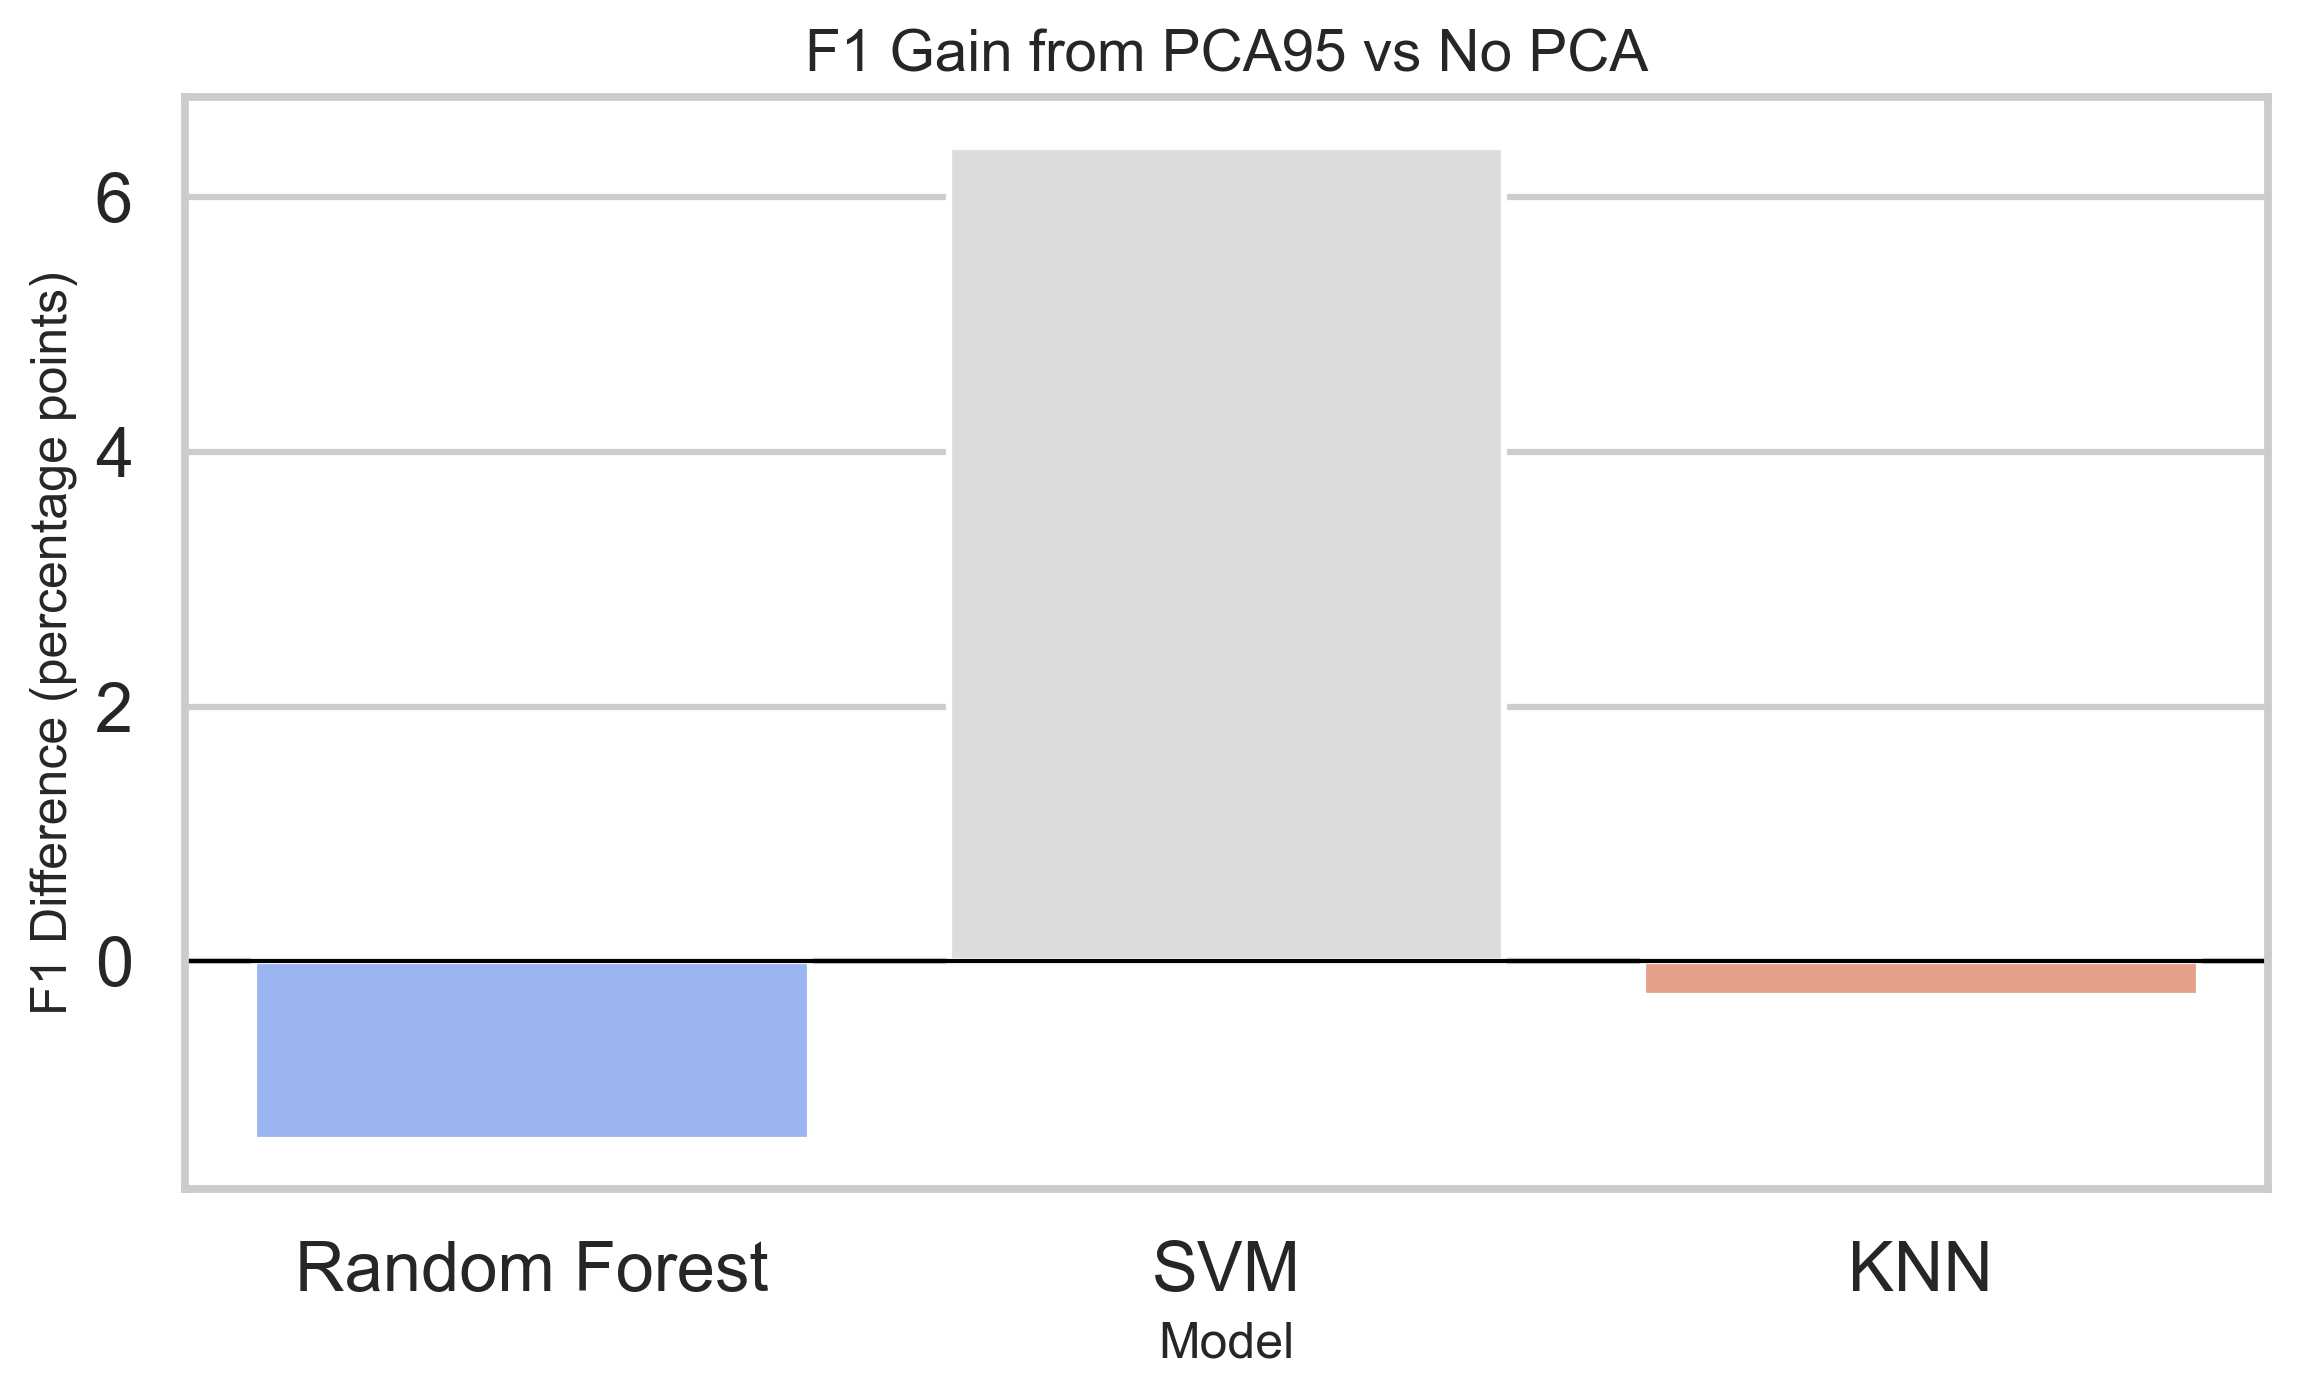
\includegraphics[width=0.85\linewidth]{Images/Generated/Chapter4/ch4_f1_gain_pca_vs_no_pca.png}
	\caption{تغییر \lr{F1} هر مدل پس از اعمال \lr{PCA95}}
	\label{fig:ch4_f1_gain_pca}
\end{figure}

\noindent\textbf{توضیح شکل:} این شکل مشخص می کند کاهش بعد برای هر مدل سودمند بوده یا باعث افت عملکرد شده است.
\vspace{0.8em}



\subsection{تحلیل ویژگی‌های مؤثر}

اگرچه مدل‌های یادگیری ماشین قادر به انجام پیش‌بینی با دقت مناسب هستند، اما بررسی ویژگی‌های مؤثر در تصمیم‌گیری مدل می‌تواند در تفسیر نتایج نیز مفید باشد. به همین منظور اهمیت ویژگی‌ها در مدل
 \lr{Random Forest}
 مورد بررسی قرار گرفت.

به منظور افزایش قابلیت تفسیر نتایج، علاوه بر ارزیابی عملکرد مدل‌ها، اهمیت نسبی ویژگی‌های استخراج‌شده نیز بررسی شد. این تحلیل مشخص می‌کند که تصمیم‌گیری مدل تا چه اندازه به هر یک از ویژگی‌های سینماتیکی وابسته بوده است.


\begin{figure}[H]
	\centering
	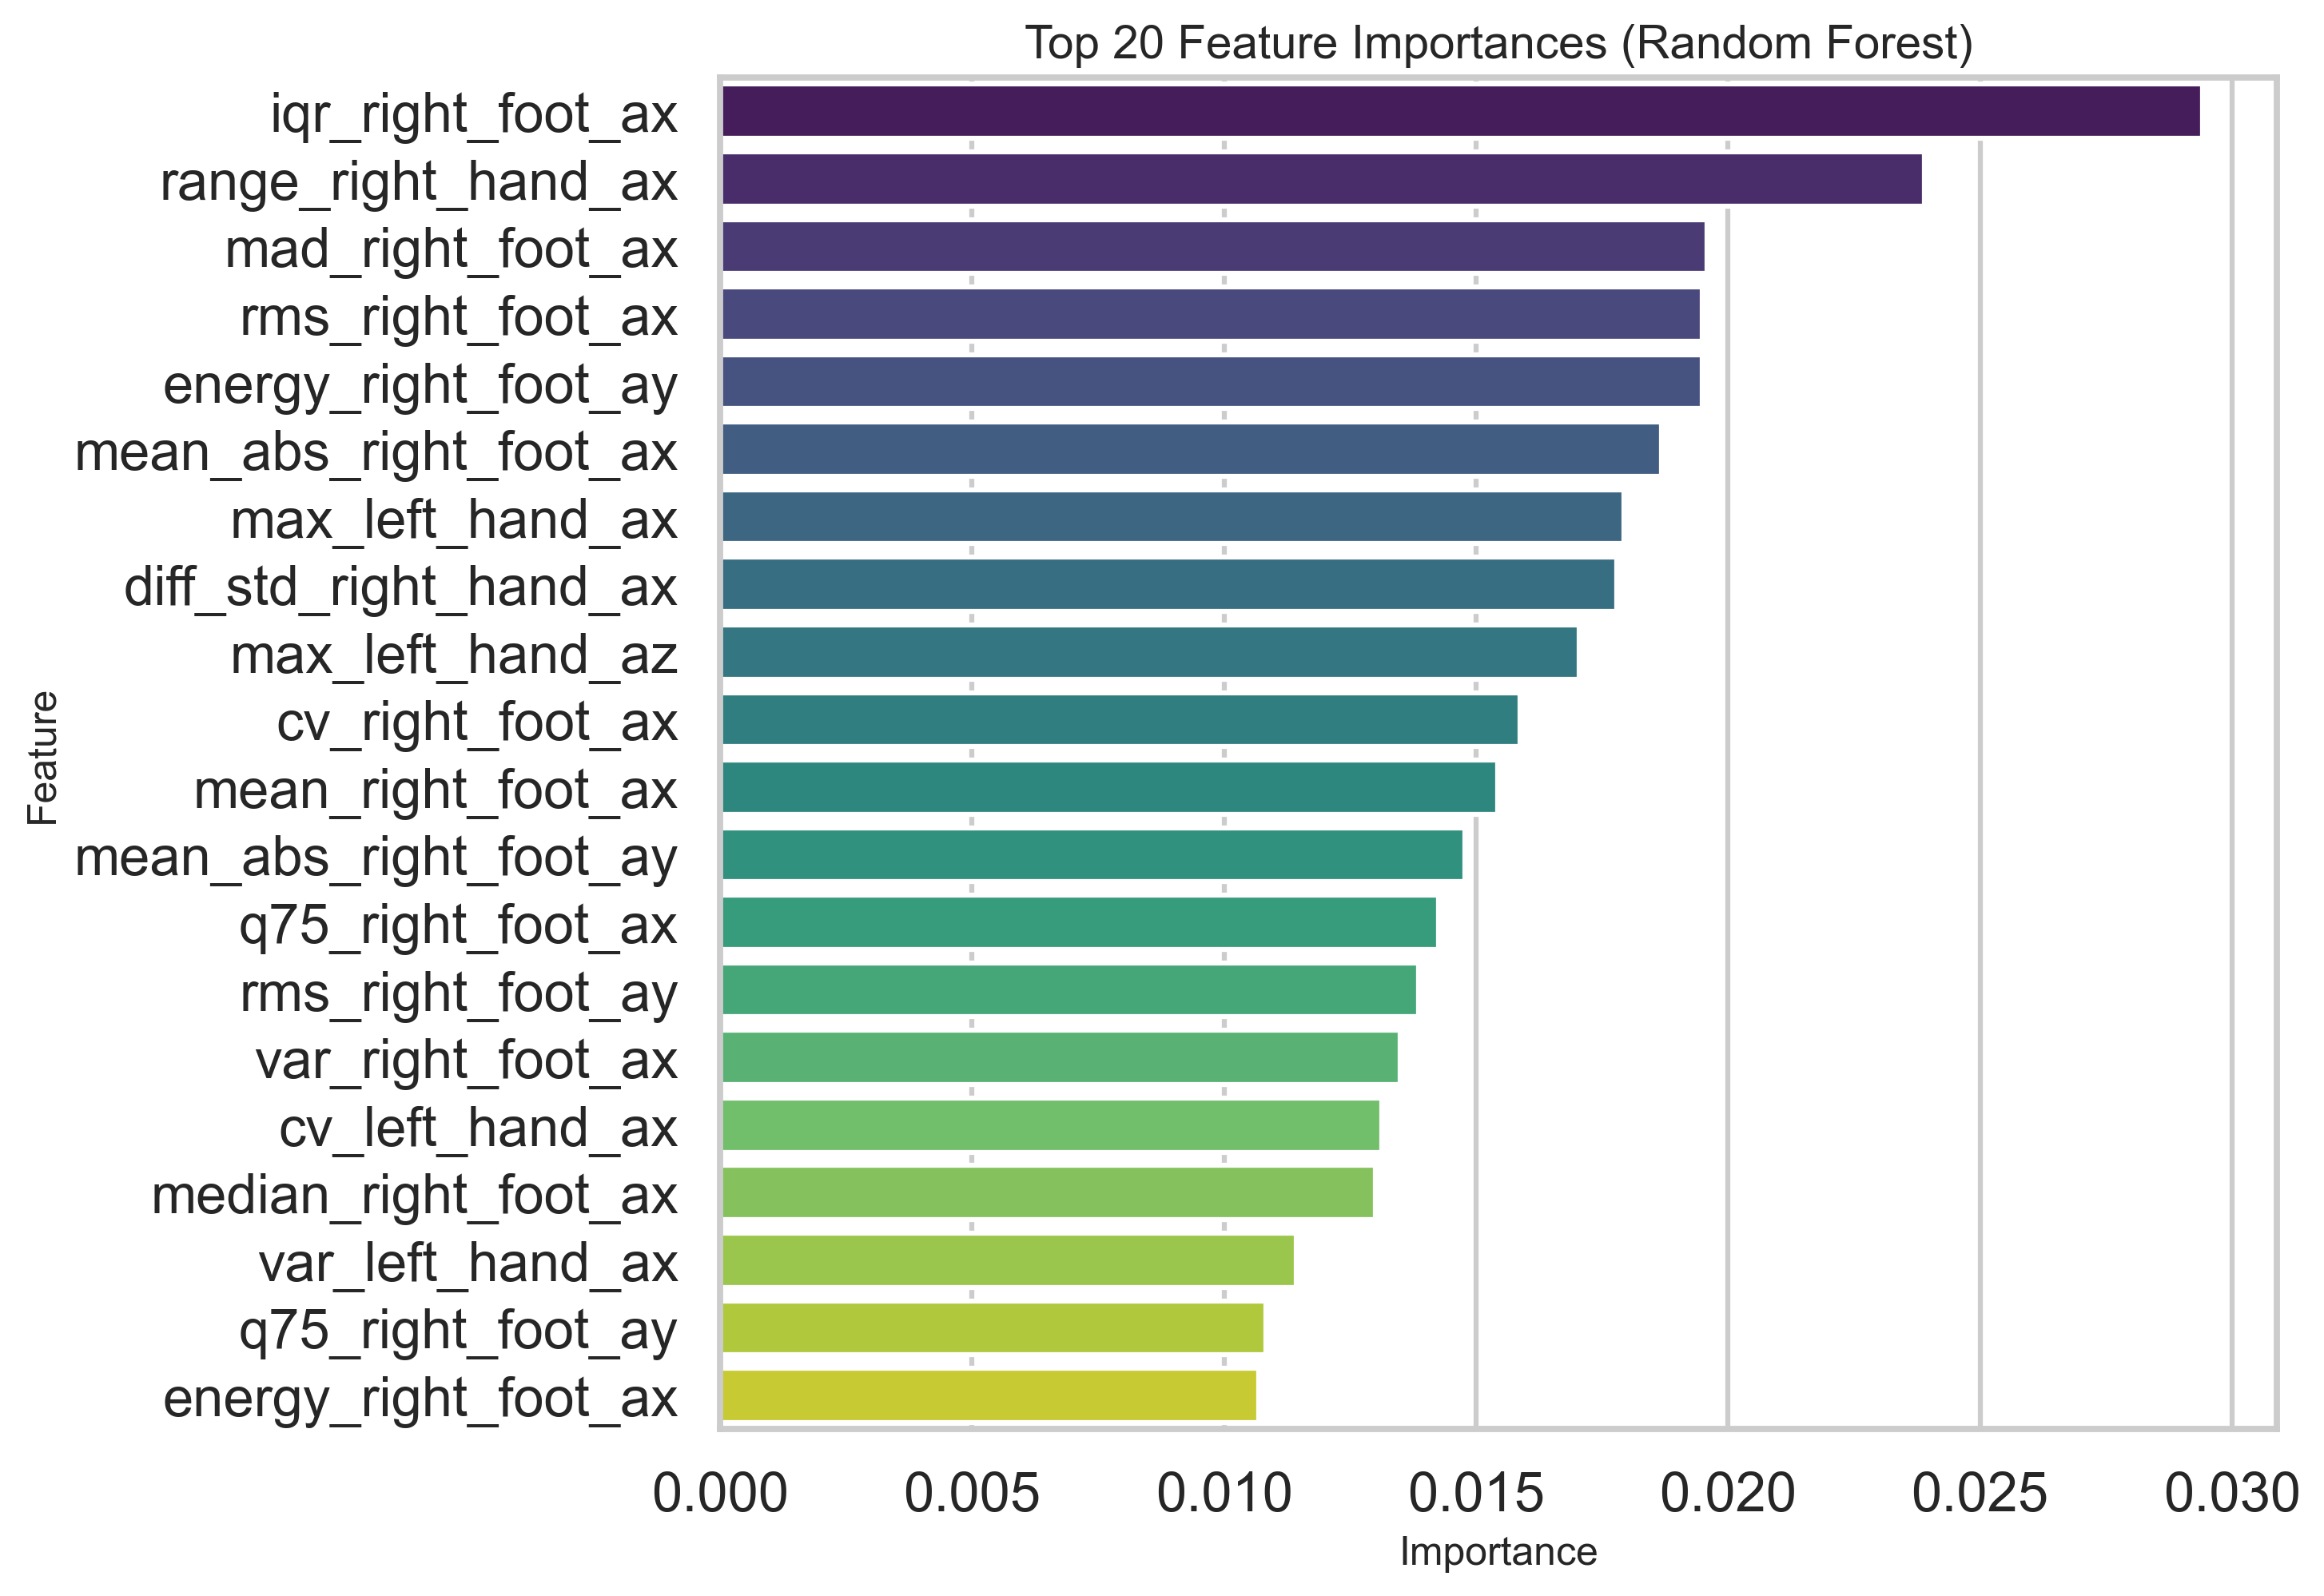
\includegraphics[width=0.85\linewidth]{Images/Generated/Chapter4/ch4_rf_top_feature_importance.png}
	\caption{20 ویژگی برتر بر اساس اهمیت در مدل \lr{Random Forest}}
	\label{fig:ch4_rf_importance}
\end{figure}

\noindent\textbf{توضیح شکل:} این شکل نشان می دهد کدام ویژگی ها نقش بیشتری در تصمیم گیری مدل داشته اند و برای تفسیر بالینی/مهندسی مفید است.
\vspace{0.8em}

\begin{figure}[H]
	\centering
	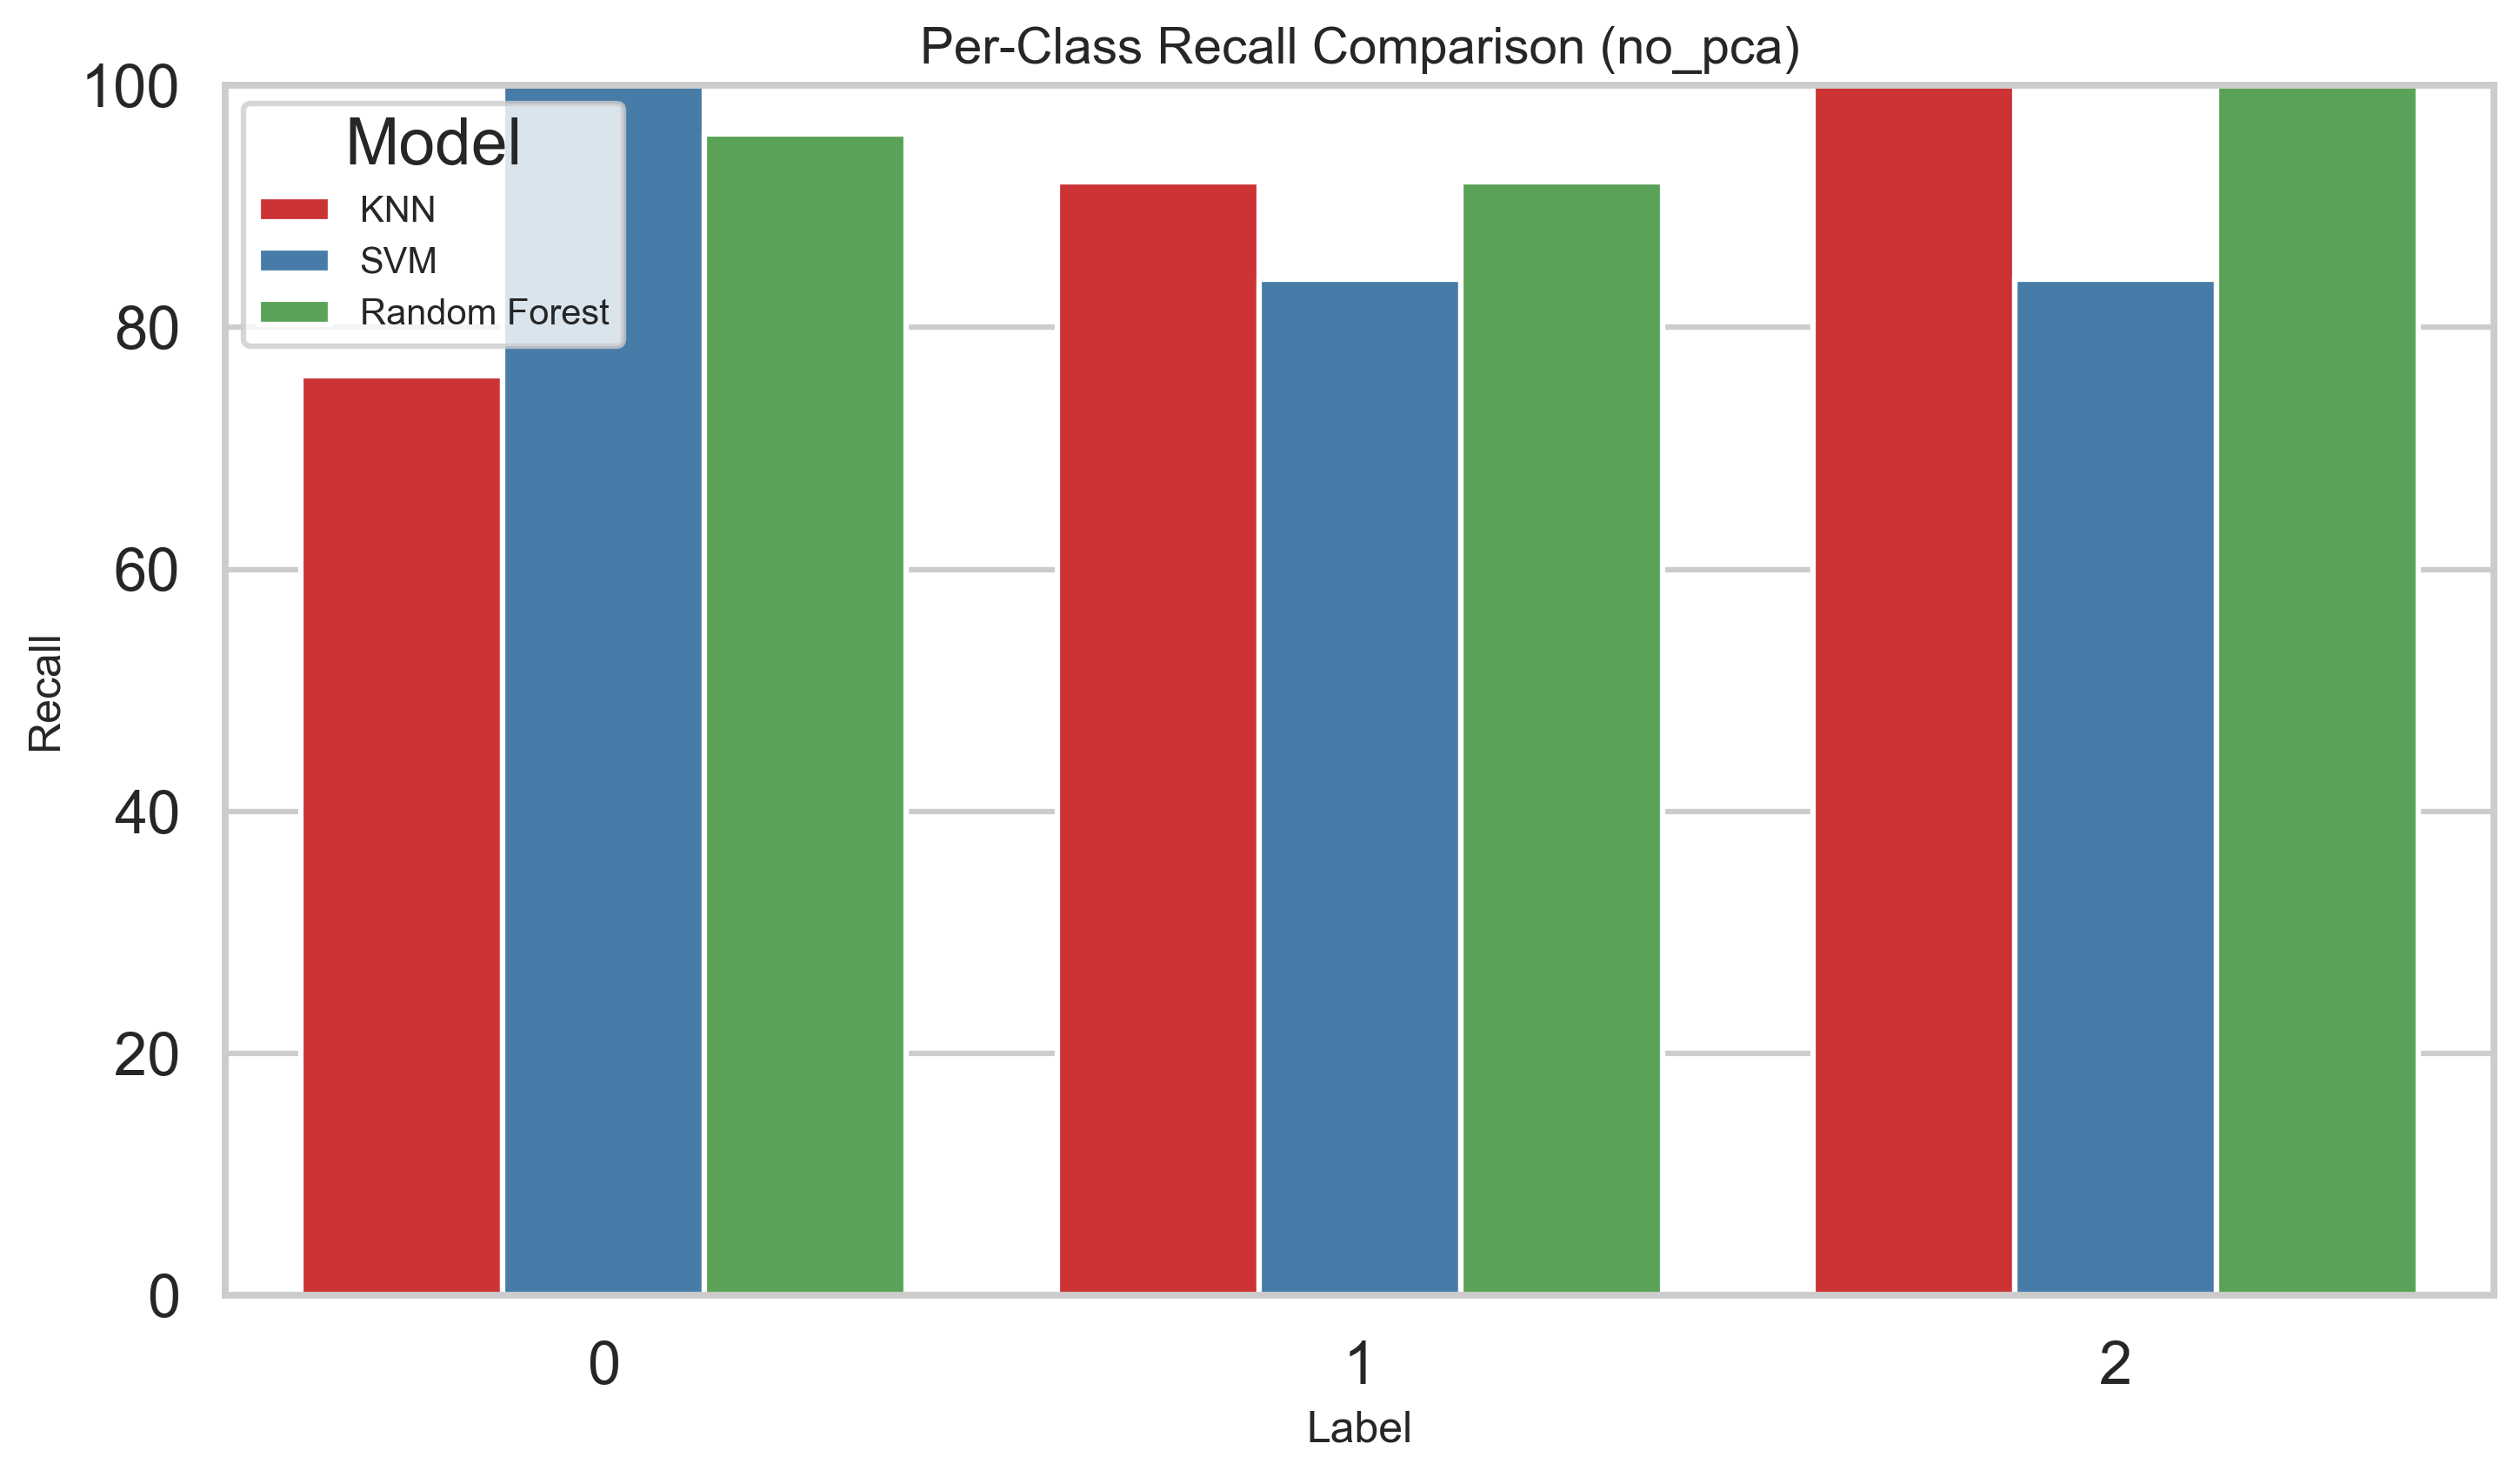
\includegraphics[width=0.85\linewidth]{Images/Generated/Chapter4/ch4_per_class_recall_no_pca.png}
	\caption{مقایسه \lr{Recall} هر کلاس بین مدل ها \lr{no pca}}
	\label{fig:ch4_per_class_recall_no_pca}
\end{figure}

\noindent\textbf{توضیح شکل:} این نمودار حساسیت هر مدل نسبت به هر کلاس را نشان می دهد و برای تحلیل خطاهای کلاس محور استفاده می شود.
\vspace{0.8em}


\begin{figure}[H]
	\centering
	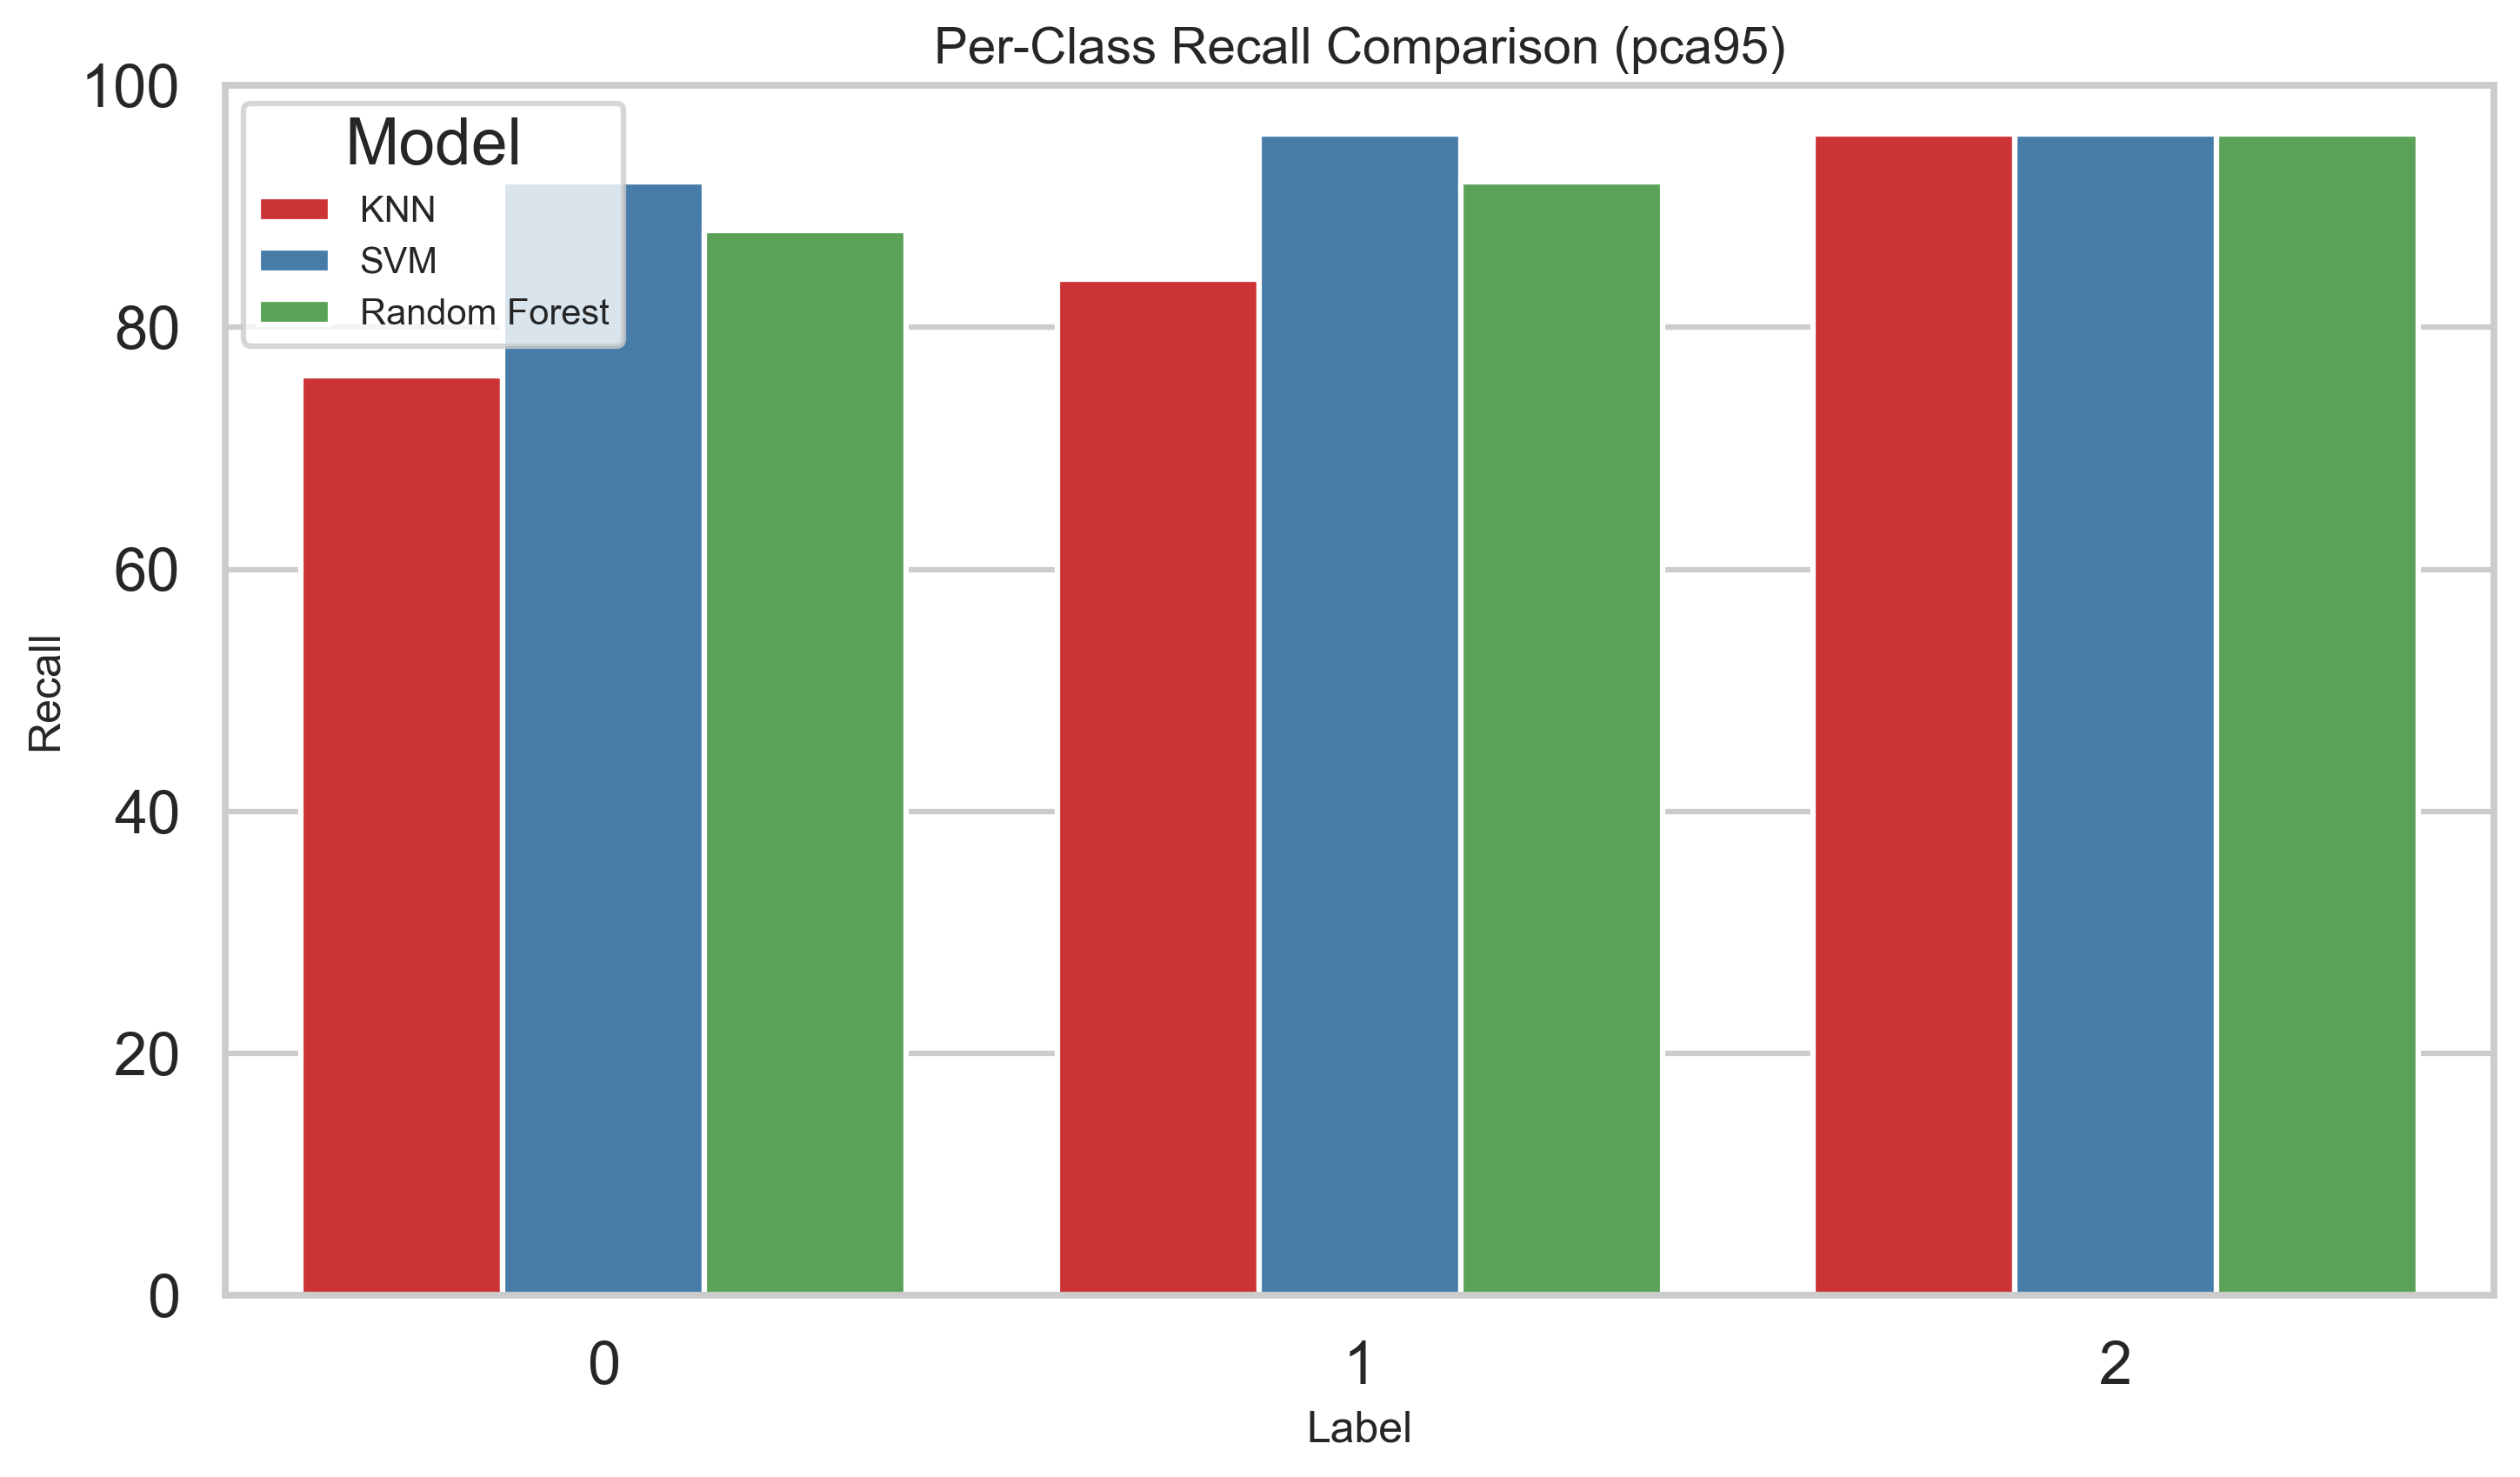
\includegraphics[width=0.85\linewidth]{Images/Generated/Chapter4/ch4_per_class_recall_pca95.png}
	\caption{مقایسه \lr{Recall} هر کلاس بین مدل ها \lr{pca95}}
	\label{fig:ch4_per_class_recall_pca95}
\end{figure}

\noindent\textbf{توضیح شکل:} این نمودار حساسیت هر مدل نسبت به هر کلاس را نشان می دهد و برای تحلیل خطاهای کلاس محور استفاده می شود.
\vspace{0.8em}


\begin{figure}[H]
	\centering
	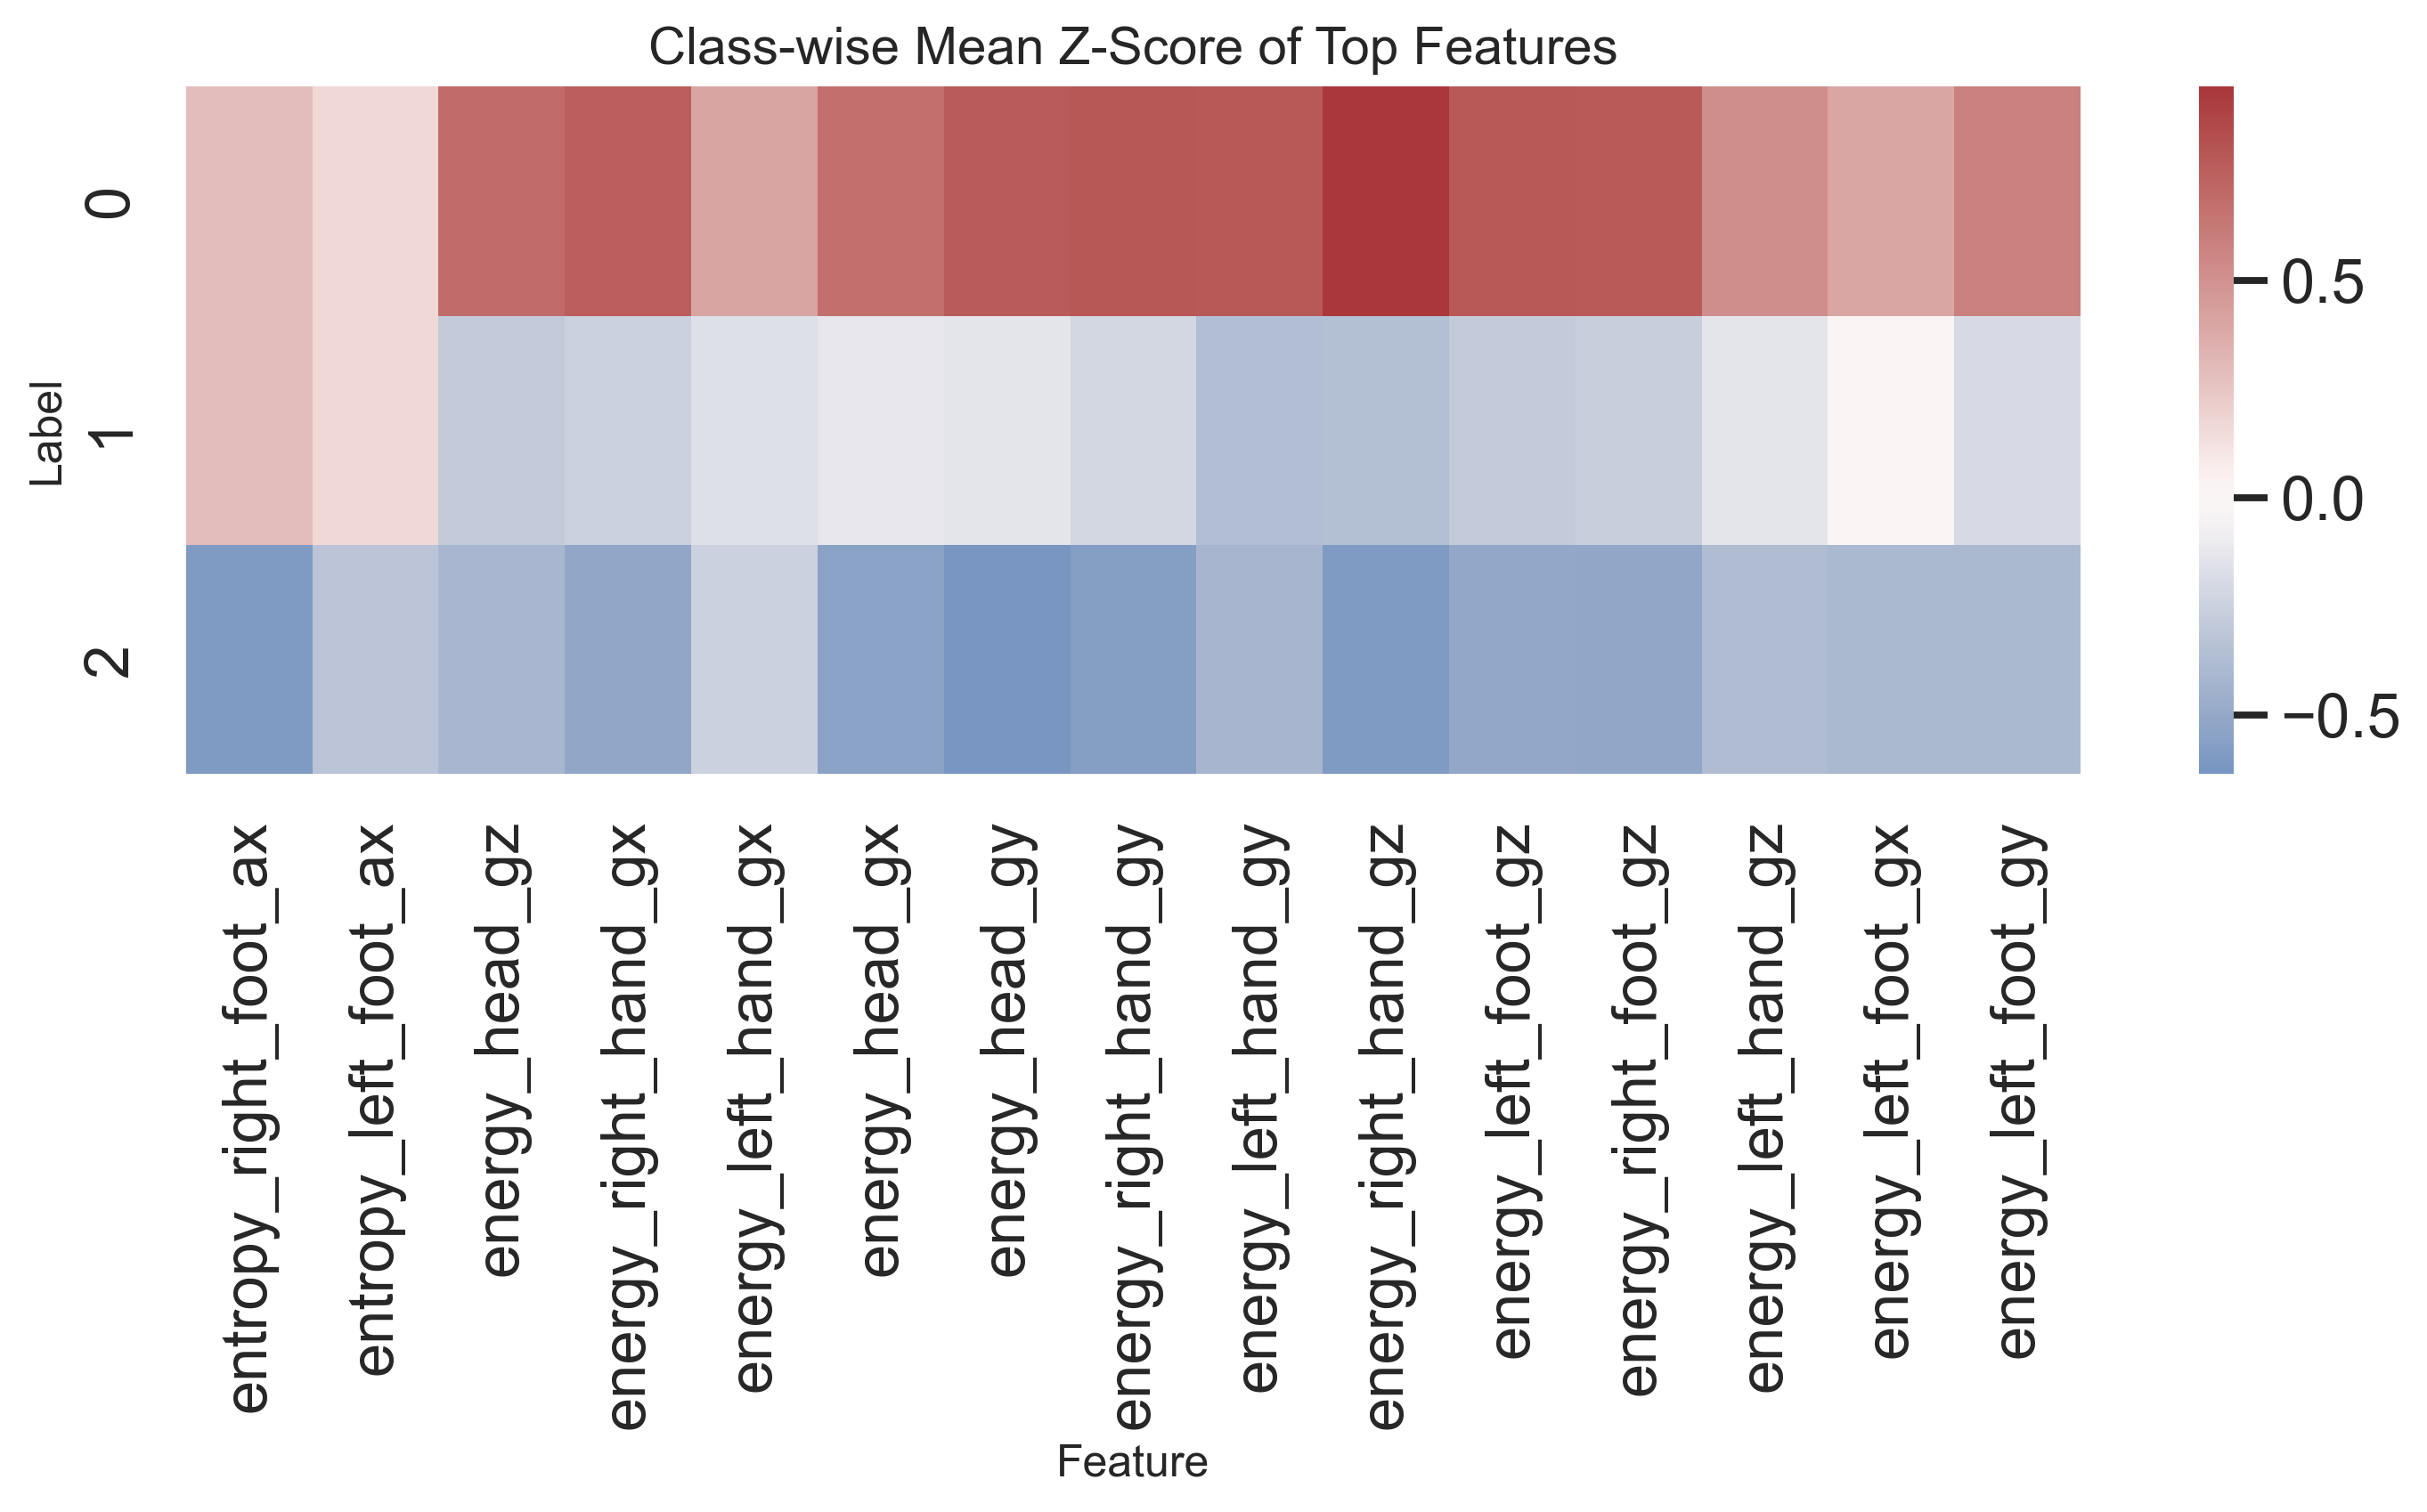
\includegraphics[width=0.85\linewidth]{Images/Generated/Chapter4/ch4_class_centroid_feature_heatmap.png}
	\caption{میانگین نرمال شده ویژگی های برتر برای هر کلاس}
	\label{fig:ch4_class_centroid_heatmap}
\end{figure}

\noindent\textbf{توضیح شکل:} این نقشه حرارتی الگوی میانگین ویژگی ها در کلاس های مختلف را نشان می دهد و قابلیت تفکیک ویژگی ها را تفسیرپذیر می کند.
\vspace{0.8em}


\subsection{جمع‌بندی فصل}

نتایج این فصل نشان داد که سامانه پیشنهادی قادر به ثبت داده‌های حرکتی با کیفیت مناسب و استخراج ویژگی‌های مؤثر از سیگنال‌های حسگرهای اینرسیایی است. بررسی عملکرد مدل‌های مختلف یادگیری ماشین نیز نشان داد که ویژگی‌های استخراج‌شده توانایی مناسبی در تفکیک کلاس‌های مختلف فعالیت دارند.

همچنین مشخص شد که استفاده از روش کاهش بعد 
\lr{PCA}
 بسته به نوع الگوریتم می‌تواند موجب بهبود یا افت عملکرد شود؛ بنابراین انتخاب استفاده از 
 \lr{PCA}
  باید متناسب با مدل مورد استفاده انجام گیرد. علاوه بر این، تحلیل اهمیت ویژگی‌ها نشان داد که تنها بخشی از ویژگی‌های استخراج‌شده نقش اصلی را در فرآیند تصمیم‌گیری مدل‌ها ایفا می‌کنند که این موضوع می‌تواند در طراحی سامانه‌های ساده‌تر و کارآمدتر در آینده مورد استفاده قرار گیرد.

در مجموع، نتایج به‌دست‌آمده نشان می‌دهد که ترکیب حسگرهای اینرسیایی پوشیدنی با روش‌های پردازش سیگنال و الگوریتم‌های یادگیری ماشین، رویکردی مناسب برای تحلیل فعالیت‌های عملکردی و پیش‌بینی وضعیت حرکتی بیماران مبتلا به دیستروفی عضلانی دوشن فراهم می‌کند.







